% ---------------------------------------------------------------
% TEMPLATE TCC1 - SENAC SANTO AMARO
% ---------------------------------------------------------------
% Trabalho de Conclusão de Curso 1
% Elaborado para apresentação da proposta inicial do TCC
% Estrutura: 4 capítulos (Introdução, Revisão Bibliográfica,
%            Desenvolvimento, Referências Bibliográficas)
% ---------------------------------------------------------------

\documentclass[
    12pt,                % tamanho da fonte
    openright,           % capítulos começam em página ímpar
    oneside,             % para impressão em apenas um lado do papel
    a4paper,             % tamanho do papel
    english,             % idioma adicional
    brazil               % idioma principal
]{abntex2}

% ---------------------------------------------------------------
% PACOTES
% ---------------------------------------------------------------
\usepackage{lmodern}                % Fonte Latin Modern
\usepackage[T1]{fontenc}            % Seleção de códigos de fonte
\usepackage[utf8]{inputenc}         % Codificação do documento
\usepackage{lastpage}               % Usado pela Ficha catalográfica
\usepackage{indentfirst}            % Indenta o primeiro parágrafo
\usepackage{color}                  % Controle de cores
\usepackage{graphicx}               % Inclusão de gráficos
\usepackage{microtype}              % Melhorias de justificação
\usepackage{float}                  % Para posicionamento de figuras
\usepackage{booktabs}               % Tabelas profissionais
\usepackage{multirow}               % Células mescladas em tabelas
\usepackage{longtable}              % Tabelas longas
\usepackage{amsmath,amssymb}        % Símbolos matemáticos
\usepackage{pgfgantt}               % Diagramas de Gantt
\usepackage[brazilian,hyperpageref]{backref}  % Páginas com citações
\usepackage[alf]{abntex2cite}       % Citações ABNT
\usepackage{tabularx}
\usepackage{booktabs}
\usepackage{placeins}

% ---------------------------------------------------------------
% CONFIGURAÇÕES DO PDF
% ---------------------------------------------------------------
\makeatletter
\hypersetup{
    pdftitle={\@title},
    pdfauthor={\@author},
    pdfsubject={TCC1 - SENAC Santo Amaro},
    pdfcreator={LaTeX with abnTeX2},
    pdfkeywords={tcc}{senac}{santo amaro}{trabalho de conclusão},
    colorlinks=true,        % false: links em caixas; true: links coloridos
    linkcolor=blue,         % cor dos links internos
    citecolor=blue,         % cor dos links para bibliografia
    filecolor=magenta,      % cor dos links para arquivos
    urlcolor=blue,
    bookmarksdepth=4
}
\makeatother

% ---------------------------------------------------------------
% CONFIGURAÇÕES DE APARÊNCIA DO PDF FINAL
% ---------------------------------------------------------------
\definecolor{blue}{RGB}{41,5,195}

% ---------------------------------------------------------------
% INFORMAÇÕES DO DOCUMENTO
% ---------------------------------------------------------------
\titulo{Detecção de Ataques DDoS em Redes de Computadores utilizando Algoritmos Supervisionados de Machine Learning: uma Análise Comparativa entre Random Forest e Support Vector Machine}
\autor{Bianca Lima Rodrigues e Bruno José Oliveira Gomes}
\local{São Paulo}
\data{2026}
\orientador{Prof. Afonso Cesar Lelis Brandão}
% \coorientador{Prof. Nome do Coorientador} % Descomente se houver coorientador

\instituicao{%
  SENAC -- Serviço Nacional de Aprendizagem Comercial
  \par
  Unidade Santo Amaro
  \par
  Curso de Ciência da computação
}

\tipotrabalho{Trabalho de Conclusão de Curso I}

\preambulo{Proposta de Trabalho de Conclusão de Curso apresentado ao SENAC Santo Amaro como requisito parcial para aprovação na disciplina de TCC1 do curso de Ciência da computação.}

% ---------------------------------------------------------------
% COMPILA O ÍNDICE
% ---------------------------------------------------------------
\makeindex

% ---------------------------------------------------------------
% INÍCIO DO DOCUMENTO
% ---------------------------------------------------------------
\begin{document}

% Seleciona o idioma do documento
\selectlanguage{brazil}

% Retira espaço extra obsoleto entre as frases
\frenchspacing

% ---------------------------------------------------------------
% ELEMENTOS PRÉ-TEXTUAIS
% ---------------------------------------------------------------
\pretextual

% ---------------------------------------------------------------
% CAPA
% ---------------------------------------------------------------
\imprimircapa

% ---------------------------------------------------------------
% FOLHA DE ROSTO
% ---------------------------------------------------------------
\imprimirfolhaderosto

% ---------------------------------------------------------------
% RESUMO
% ---------------------------------------------------------------
% \begin{resumo}
% Este documento apresenta a proposta inicial do Trabalho de Conclusão de Curso (TCC1) desenvolvido no SENAC Santo Amaro. O objetivo deste trabalho é treinar e comparar diferentes algoritmos supervisionados de Machine Learning, como Random Forest, Support Vector Machine e Multi-Layer Perceptron, para a detecção de intrusões em redes de computadores. A justificativa para este estudo baseia-se no crescimento significativo de ataques cibernéticos e na necessidade de soluções mais eficazes para identificação de atividades maliciosas em tempo real.

% A revisão bibliográfica abrange temas como detecção de intrusão, segurança em redes de computadores e aplicação de algoritmos de aprendizado de máquina para identificação de anomalias. Como solução proposta, pretende-se desenvolver uma abordagem experimental baseada no treinamento e validação de modelos utilizando conjuntos de dados de tráfego de rede, avaliando seu desempenho por meio de métricas como acurácia, precisão, recall e F1-score.

% Este trabalho está organizado em três capítulos que apresentam a introdução ao tema, a revisão bibliográfica que fundamenta a pesquisa, o desenvolvimento com a solução proposta e o cronograma de trabalho, seguidos das referências bibliográficas.


% \vspace{\onelineskip}

% \noindent
% \textbf{Palavras-chave}: detecção de intrusão, machine learning, redes de computadores, análise comparativa, random forest.
% \end{resumo}

% ---------------------------------------------------------------
% LISTA DE ILUSTRAÇÕES
% ---------------------------------------------------------------
% \pdfbookmark[0]{\listfigurename}{lof}
% \listoffigures*
% \cleardoublepage

% ---------------------------------------------------------------
% LISTA DE TABELAS
% ---------------------------------------------------------------
% \pdfbookmark[0]{\listtablename}{lot}
% \listoftables*
% \cleardoublepage

% ---------------------------------------------------------------
% SUMÁRIO
% ---------------------------------------------------------------
\pdfbookmark[0]{\contentsname}{toc}
\tableofcontents*
\cleardoublepage

% ---------------------------------------------------------------
% ELEMENTOS TEXTUAIS
% ---------------------------------------------------------------
\textual

% ===============================================================
% CAPÍTULO 1 - INTRODUÇÃO
% ===============================================================
\chapter{Introdução}
\label{cap:introducao}

Segundo a \citeonline{CheckPoint2026}, no relatório anual Cyber Security Report 2026, as organizações sofreram, em média, 1.968 ataques cibernéticos semanais em 2025, representando um aumento de 70\% em relação a 2023, impulsionado principalmente pelo uso de Inteligência Artificial e automação por atacantes. Segundo a pesquisa, em fevereiro de 2026, o número médio de ataques cibernéticos semanais por organização aumentou 9,6\% em relação ao ano anterior, evidenciando a crescente vulnerabilidade das redes de computadores \cite{CheckPoint2026}.
Esse cenário reforça a necessidade da utilização de métodos de detecção de intrusões, para a proteção de sistemas e dados, além de mitigar riscos e prevenir ataques.
A utilização de algoritmos supervisionados de Machine Learning para a detecção de anomalias em redes, surge como uma alternativa promissora para identificar atividades maliciosas em tempo real, permitindo uma análise de ataques DDoS (Distributed Denial of Service).
Este trabalho tem como objetivo geral comparar dois modelos diferentes de Machine Learning, sendo o Random Forest e o Support Vector Machine. A partir disso, busca-se avaliar a eficiência desses algoritmos na detecção de intrusões em redes de computadores, utilizando algoritmos supervisionados, através da classificação binária, para distinguir o tráfego de rede entre o normal e anômalo.
Será utilizado para atingir os objetivos propostos o conjunto de dados CICDDoS2019, que contém dados de tráfego normal e malicioso, além disso, será adotada uma metodologia experimental, considerada adequada para a realização de comparações e medições de desempenho entre os modelos. A análise será conduzida com base em métricas como acurácia, precisão, recall, F1-score e Coeficiente de correlação de Matthews (MCC) possibilitando uma avaliação consistente dos resultados obtidos.

A Figura 1 apresenta a evolução da quantidade de ataques cibernéticos registrados nos cinco países mais visados da América Latina ao longo de 2025. Observa-se que o Brasil se destaca significativamente em relação aos demais países da região, mantendo o maior volume de ocorrências durante todo o período analisado. Esses dados evidenciam a relevância do cenário brasileiro no contexto das ameaças cibernéticas e reforçam a necessidade de pesquisas voltadas ao desenvolvimento de mecanismos eficientes para detecção e mitigação de ataques em redes de computadores. 

\begin{figure}[h]
    \centering
    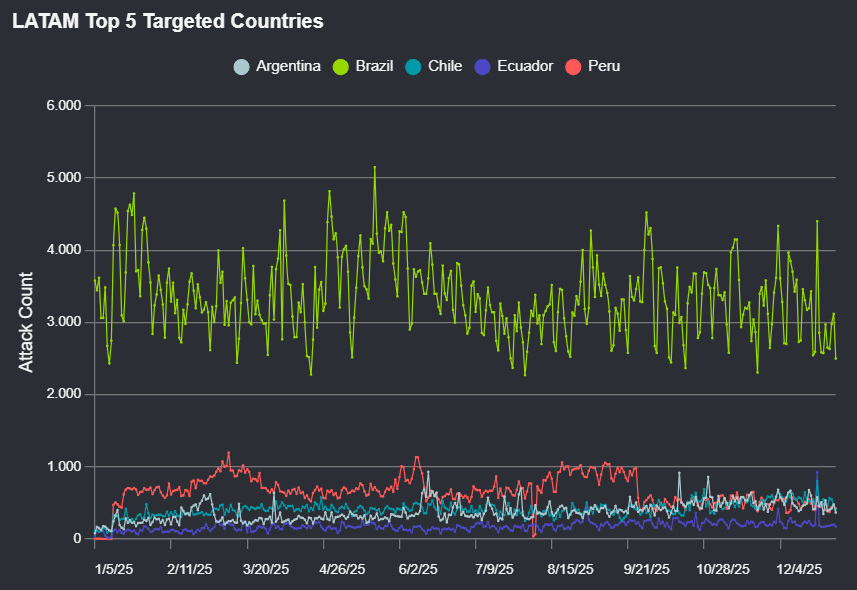
\includegraphics[width=0.90\textwidth]{ataquesLATAM.png}
    \caption{Relatório de Inteligência de Ameaças DDoS  - LATAM}
    \legend{Fonte: \citeonline{NETSCOUT2025}}
\end{figure}

\FloatBarrier




% ---------------------------------------------------------------
\section{Contexto}
\label{sec:contexto}
A crescente dependência de serviços digitais em setores como comércio, educação, saúde e administração pública tem ampliado significativamente a exposição de sistemas computacionais a ameaças cibernéticas, entre elas os ataques distribuídos de negação de serviço (Distributed Denial-of-Service – DDoS). Esse tipo de ataque tem se destacado pelo aumento de frequência e complexidade, sendo caracterizado pela sobrecarga intencional de servidores, aplicações ou redes por meio do envio massivo de tráfego oriundo de múltiplas fontes comprometidas, com o objetivo de tornar serviços indisponíveis para usuários legítimos \cite{IBM2026}. Segundo a \citeonline{Cloudflare2025}, o crescimento contínuo desses ataques evidencia a ampliação do risco para organizações de diferentes setores, afetando diretamente empresas, instituições públicas e usuários finais. Entre as principais consequências estão a interrupção de serviços essenciais, prejuízos financeiros, danos à reputação institucional e comprometimento da confiança nos ambientes digitais.
Nesse cenário, torna-se evidente a necessidade de aprimorar os mecanismos de defesa atualmente utilizados, uma vez que métodos tradicionais de detecção nem sempre conseguem acompanhar a evolução das técnicas empregadas pelos atacantes. De acordo com a \citeonline{Cloudflare2025}, os ataques DDoS vêm se tornando cada vez mais sofisticados e volumosos, exigindo soluções capazes de identificar padrões anômalos em tempo real e responder rapidamente às ameaças. Conforme destaca a \citeonline{IBM2026}, a mitigação eficaz desses ataques depende da adoção de estratégias automatizadas e inteligentes que fortaleçam a resiliência das infraestruturas digitais. Dessa forma, o uso de técnicas de Machine Learning aplicadas à detecção de intrusão surge como uma alternativa promissora para aumentar a capacidade de prevenção e resposta a ataques DDoS, contribuindo para a proteção da disponibilidade e da segurança dos serviços digitais essenciais à sociedade.

% \vspace{0.3cm}
% \noindent\fbox{\parbox{\dimexpr\textwidth-2\fboxsep-2\fboxrule}{%
% \textbf{Orientação sobre citações (ABNT NBR 10520:2023)}

% \vspace{0.2cm}
% O aluno deve \textbf{priorizar citações indiretas} (paráfrases), nas quais a ideia do autor é reescrita com as próprias palavras. Citações diretas (transcrições literais) \textbf{não são recomendadas}, exceto quando o texto original for insubstituível --- por exemplo, definições consagradas, leis, normas técnicas ou trechos cuja reformulação alteraria o sentido.

% \vspace{0.2cm}
% \textbf{Citação indireta} (recomendada) --- o autor interpreta e reescreve a ideia:

% \vspace{0.1cm}
% \textit{Exemplo 1 --- sistema autor-data entre parênteses:}\\
% A definição clara do problema é considerada um fator determinante para o sucesso de qualquer pesquisa na área de Computação \cite{Wazlawick2020}.

% \vspace{0.1cm}
% \textit{Exemplo 2 --- autor como parte do texto:}\\
% Para \citeonline{Pressman2016}, a escolha de uma metodologia adequada impacta diretamente na qualidade dos resultados obtidos em projetos de software.

% \vspace{0.2cm}
% \textbf{Citação direta curta} (até 3 linhas, apenas quando indispensável) --- entre aspas, com indicação de página:

% \vspace{0.1cm}
% Segundo \citeonline[p.~42]{Wazlawick2020}, ``a formulação do problema deve ser expressa de forma clara, objetiva e delimitada, evitando ambiguidades que possam comprometer o escopo da pesquisa''.

% \vspace{0.2cm}
% \textbf{Citação direta longa} (mais de 3 linhas, apenas quando indispensável) --- recuo de 4\,cm, fonte menor, sem aspas:

% \begin{citacao}
% A revisão bibliográfica não consiste em simplesmente listar os trabalhos encontrados, mas em analisá-los criticamente, identificando convergências, divergências e lacunas que justifiquem a realização de uma nova pesquisa \cite[p.~87]{Wazlawick2020}.
% \end{citacao}

% \textbf{Resumo}: use citações indiretas como regra. Reserve a citação direta para casos excepcionais em que a transcrição literal seja realmente necessária.
% }}

% ---------------------------------------------------------------
\section{Justificativa}
\label{sec:justificativa}

Com a evolução da infraestrutura da inteligência artificial e o aumento da complexidade dos ambientes computacionais, os ataques cibernéticos, especialmente os ataques distribuídos de negação de serviço (DDoS), têm se tornado mais sofisticados, frequentes e difíceis de mitigar, exigindo soluções cada vez mais rápidas e inteligentes para sua detecção \cite{Thaqi2026}. Esses ataques comprometem a disponibilidade de serviços essenciais ao sobrecarregar recursos computacionais e de rede, gerando prejuízos operacionais, financeiros e reputacionais para organizações públicas e privadas \cite{Ouhssini2024}. Casos amplamente divulgados, como o ataque do tipo Distributed Reflective Denial of Service (DRDoS) direcionado à infraestrutura da Amazon Web Services (AWS), evidenciam como eventos dessa natureza podem afetar diretamente milhões de usuários e reforçam a importância do desenvolvimento de mecanismos capazes de detectar e responder rapidamente a esse tipo de ameaça \cite{Subramani2020}.
 
Diferentemente das abordagens tradicionais baseadas em assinaturas, os modelos de aprendizado de máquina possibilitam a análise de grandes volumes de dados e a identificação de padrões anômalos, permitindo maior
capacidade de adaptação frente à constante evolução dos ataques cibernéticos \cite{Ouhssini2024}. 

\begin{itemize}
    \item \textbf{Relevância acadêmica}:Sob a perspectiva acadêmica, este trabalho contribui para o avanço das pesquisas na interseção entre segurança da informação e inteligência artificial, explorando técnicas de aprendizado de máquina aplicadas especificamente à detecção de ataques DDoS e ampliando a compreensão sobre sua eficácia em cenários reais, nos quais a literatura recente aponta a necessidade crescente de mecanismos de defesa mais robustos e adaptáveis \cite{Ouhssini2024}.
    \item \textbf{Relevância prática/profissional}: Do ponto de vista prático e profissional, o desenvolvimento de modelos inteligentes para detecção de intrusão pode proporcionar benefícios significativos, como a redução do tempo de resposta a incidentes, a identificação mais precisa de padrões maliciosos e o aumento da disponibilidade de serviços críticos para empresas e usuários \cite{Tandon2020}. 
    \item \textbf{Lacuna identificada}: Embora modelos de linguagem de grande porte (LLMs) possam analisar logs de segurança e padrões de tráfego de rede para identificar anomalias e prever ataques também, há pontos que precisam ser considerados antes de sua utilização. Seu elevado custo computacional e energético ainda representa uma limitação importante, tornando algoritmos tradicionais de machine learning, como Random Forest e Support Vector Machine, alternativas mais viáveis e economicamente eficientes para tarefas específicas de classificação e detecção de anomalias \cite{Zschache2026}. Dessa forma, justifica-se a realização deste estudo como uma contribuição significativa para o aprimoramento dos sistemas de detecção de intrusão baseados em aprendizado de máquina.
\end{itemize}

% ---------------------------------------------------------------
\section{Objetivo}
\label{sec:objetivo}

O objetivo deste trabalho visa identificar qual o melhor desempenho entre dois modelos diferentes de aprendizado de máquina, no quesito detecção de ataques DDoS em redes de computadores.

\subsection{Objetivo principal}

Comparar e analisar dois modelos diferentes supervisionados de Machine Learning: Random Forest e Support Vector Machine, avaliando suas eficácias na identificação de ataques DDoS em redes de computadores.

\subsection{Objetivos secundários}

\begin{enumerate}
    \item  Realizar levantamento bibliográfico sobre sistema detecção de intrusão em redes, ataques DDoS e aplicação de algoritmos de Machine Learning em segurança de redes;
    \item Realizar o pré-processamento do conjunto de dados escolhido, CICDDoS2019, com o intuito de garantir a consistência dos dados;
    \item Implementar, treinar e testar a desenvoltura dos algoritmos Random Forest e Support Vector Machine na classificação de tráfegos maliciosos;
    \item Avaliar e comparar os resultados obtidos dos modelos, através das métricas de acurácia, precisão, recall, F1-score e MCC.
\end{enumerate}

\section{Metodologia da pesquisa bibliográfica}
\label{sec:metodologia_pesquisa}

A pesquisa bibliográfica foi conduzida com o objetivo de reunir estudos relevantes sobre sistemas de detecção de intrusão em redes (IDS), ataques distribuídos de negação de serviço (DDoS) e a aplicação de técnicas de Machine Learning supervisionado para classificação de tráfego malicioso.

\begin{itemize}
    \item \textbf{Bases de dados consultadas}: Para isso, foram consultadas bases de dados reconhecidas na área de computação e segurança da informação, incluindo Google Scholar, IEEE Xplore, Papers with Code, Directory of Open Access Journals (DOAJ), arXiv, SciELO e Semantic Scholar, buscando garantir diversidade e qualidade das fontes analisadas.

    \item \textbf{Palavras-chave utilizadas}: As buscas foram realizadas utilizando palavras-chave em português e inglês relacionadas ao tema da pesquisa. Entre os principais termos utilizados destacam-se: “machine learning”, “aprendizado de máquina”, “supervised learning”, “aprendizado supervisionado”, “intrusion detection system”, “sistema de detecção de intrusão”, “DDoS attack detection”, “detecção de ataques DDoS”, “network anomaly detection”, “detecção de anomalias em redes”, “Random Forest”, “Support Vector Machine”, “SVM”, “artificial intelligence”, “inteligência artificial”, “cybersecurity”, “network security”, “CICDDoS2019” e “CICDDoS2019 dataset”. A combinação desses termos permitiu localizar estudos que abordassem diretamente a aplicação de algoritmos supervisionados na identificação de tráfego malicioso em redes computacionais.
    \textit{Exemplos de strings de busca utilizadas:}

    \begin{itemize}

        \item \textbf{Google Scholar}
        
    \begin{verbatim}
    ("DDoS attack detection" OR "detecção de ataques DDoS")
    AND ("machine learning" OR "aprendizado de máquina")
    AND ("supervised learning" OR "aprendizado supervisionado")
    AND ("Random Forest" OR "Support Vector Machine" OR SVM)
    AND ("network security" OR cybersecurity)
    \end{verbatim}

        \item \textbf{IEEE Xplore}

    \begin{verbatim}
    ("intrusion detection system")
    AND ("network anomaly detection")
    AND (cybersecurity)
    AND ("CICDDoS2019")
    \end{verbatim}

        \item \textbf{arXiv}

    \begin{verbatim}
    all:"intrusion detection system"
    AND all:"Random Forest"
    \end{verbatim}

    \end{itemize}

    \item \textbf{Critérios de inclusão}: Como critérios de inclusão, foram selecionados artigos científicos, capítulos de livros e publicações técnicas em português e inglês, que apresentassem relação direta com o problema investigado, especialmente estudos envolvendo Machine Learning aplicado à detecção de intrusões e ataques DDoS, com ênfase nos algoritmos Random Forest e Support Vector Machine. Foram priorizados trabalhos com validação experimental, uso de conjuntos de dados reconhecidos na literatura, como o CICDDoS2019, e que apresentassem métricas de avaliação como acurácia, precisão, recall, F1-score e MCC.

    \item \textbf{Critérios de exclusão}: Como critérios de exclusão, foram descartados trabalhos duplicados, estudos que não abordavam diretamente os modelos de machine learning escolhidos, artigos com foco exclusivo em técnicas de aprendizado profundo sem relação com os algoritmos analisados neste trabalho, além de materiais desatualizados ou com metodologia insuficientemente descrita. Dessa forma, a pesquisa bibliográfica permitiu construir uma base teórica consistente para fundamentar o desenvolvimento experimental e a análise comparativa proposta neste estudo.

    \item \textbf{Período de abrangência}: Artigos publicados entre 2020 e 2026, salvo artigos e livros seminais ou fundamentais.
\end{itemize}

\begin{figure}[h]
    \centering
    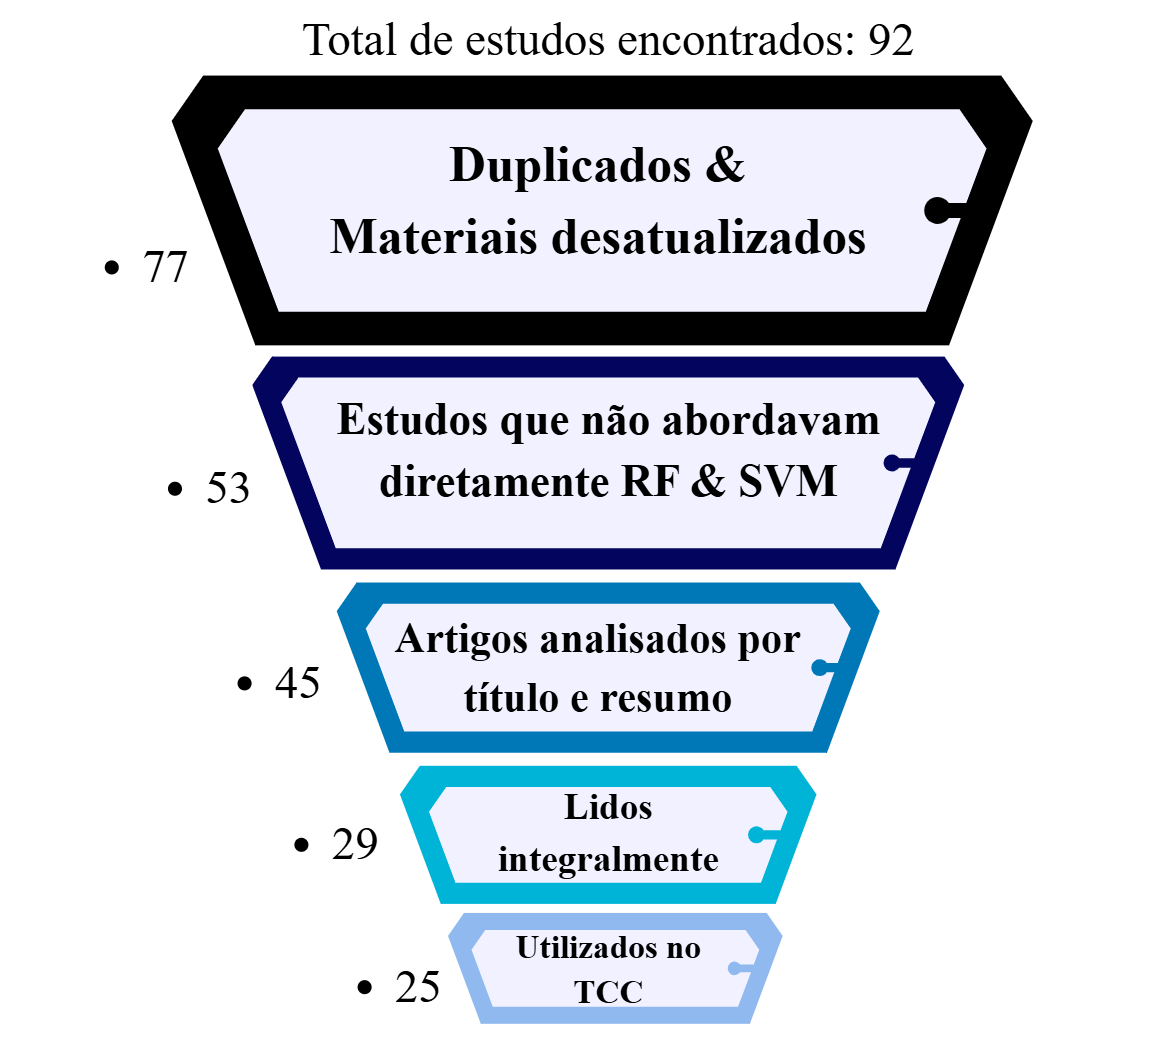
\includegraphics[width=0.75\textwidth]{filtroCriterios.png}
    \caption{Critérios de exclusão}
    \legend{Fonte: Elaborado pelo autor (2026)}
\end{figure}

\FloatBarrier


% ===============================================================
% CAPÍTULO 2 - REVISÃO BIBLIOGRÁFICA
% ===============================================================
\chapter{Revisão Bibliográfica}
\label{cap:revisao}

% ---------------------------------------------------------------
\section{Referencial teórico}
\label{sec:referencial}

\subsection{Redes de computadores}

Segundo \citeonline{Tanenbaum2011}, um conjunto de dispositivos de computação autônomos interconectados é denominado "redes de computadores", estando eles interconectados quando é possível realizar a troca de dados entre eles. A transmissão se dá através de protocolos de comunicação, que estão organizados em camadas dentro do modelo
TCP/IP.


As aplicações de redes de computadores podem ser categorizadas em Aplicações Comerciais, cujo objetivo é que os dados estejam disponíveis para qualquer pessoa na rede. Já a Aplicação Doméstica, visa abranger usuários em casa, oferecendo conectividade externa e acesso a uma vasta gama de recursos. Usuários Móveis são a categoria que utilizam rede em trânsito (em terra, mar ou ar), através de redes sem fio. E por fim, a categoria relacionada a Questões Sociais, focada para cidadãos comuns distribuírem e visualizarem conteúdos entre si \cite{Tanenbaum2011}.


As redes LAN (Local Area Network) e WAN (Wide Area Network) diferenciam-se principalmente pelo alcance geográfico. A LAN é utilizada para conectar dispositivos em áreas limitadas, como residências, escritórios e laboratórios, oferecendo maior velocidade e menor latência. Já a WAN é responsável pela interligação de diferentes redes locais em grandes distâncias, podendo abranger cidades, países ou continentes, como ocorre na internet e em redes corporativas \cite{Tanenbaum2011}.

\subsection{Protocolo}

Os dispositivos interconectados realizam a troca de informações por meio de protocolos de comunicação, definidos como um conjunto de regras e padrões que permitem a comunicação adequada entre dispositivos em uma rede. Esses protocolos são organizados em modelos de referência que estruturam as funções de comunicação em pilha de camadas. O modelo OSI é considerado um modelo teórico, utilizado como base conceitual para compreender as responsabilidades de cada camada no processo de comunicação. Em contrapartida, o modelo TCP/IP possui caráter prático, sendo amplamente utilizado na Internet e nas redes de computadores atuais para viabilizar a comunicação e a troca de dados entre diferentes sistemas \cite{Tanenbaum2011}.

\subsection{Modelo TCP/IP}

O modelo TCP/IP consiste em um conjunto de protocolos de comunicação utilizados para permitir a troca de dados entre computadores conectados em uma rede. Segundo \citeonline{Stevens1994}, a suíte TCP/IP pode ser definida como um conjunto de regras que permite a comunicação entre computadores de diferentes tamanhos, fabricantes e sistemas operacionais. Seu nome deriva de dois de seus principais protocolos: o TCP (Transmission Control Protocol) e o IP (Internet Protocol). Entretanto, a suíte TCP/IP é composta por diversos protocolos responsáveis por diferentes funções de comunicação, formando a base da Internet moderna. O desenvolvimento da arquitetura TCP/IP teve origem em pesquisas realizadas pelo Departamento de Defesa dos Estados Unidos (DoD), por meio da ARPA (Advanced Research Projects Agency), no final da década de 1960 \cite{Stevens1994}.


O modelo TCP/IP é baseado em um modelo de camadas, no qual cada camada desempenha funções específicas no processo de comunicação \cite{Stevens1994}. Essa organização em camadas facilita o desenvolvimento, a manutenção e a padronização dos protocolos de rede, além de permitir que diferentes tecnologias trabalhem de forma integrada. Nesse modelo, cada camada se comunica com sua camada equivalente em outro dispositivo por meio de protocolos específicos. Por exemplo, os protocolos da camada de transporte permitem a comunicação entre as camadas de transporte dos dispositivos conectados, em um processo conhecido como comunicação peer-to-peer. Segundo \citeonline{Stevens1994} os protocolos de rede são organizados em uma pilha de protocolos (protocol stack), onde os dados são transmitidos da camada superior para a inferior até serem enviados pelo meio físico da rede. Durante esse processo, denominado encapsulamento, cada camada adiciona informações de controle aos dados, como endereços, verificação de erros e informações de roteamento. No dispositivo receptor ocorre o processo inverso, no qual os dados sobem pelas camadas até chegarem à aplicação de destino, as informações adicionadas são removidas camada por camada, em um processo chamado desencapsulamento.
O TCP/IP é tradicionalmente dividido em quatro camadas: Aplicação, Transporte, Internet e Interface de Rede \cite{Stevens1994}.

\subsubsection{Camada de Aplicação}
A camada de Aplicação é a mais próxima do usuário e responsável pelos serviços de comunicação utilizados pelas aplicações de rede. Nela encontram-se protocolos amplamente utilizados, como HTTP (Hypertext Transfer Protocol), FTP (File Transfer Protocol), SMTP (Simple Mail Transfer Protocol), DNS (Domain Name System) e Telnet (Telecommunication Network). Essa camada realiza a interface entre os programas do usuário e os serviços de comunicação da rede \cite{Stevens1994,ESR2020}.

\subsubsection{Camada de Transporte}
A camada de Transporte é responsável pela comunicação fim a fim entre os dispositivos, garantindo controle de fluxo, integridade e confiabilidade na transmissão dos dados. Os principais protocolos dessa camada são o TCP e o UDP (User Datagram Protocol). O TCP fornece comunicação confiável e orientada à conexão, realizando controle de erros, confirmação de recebimento e retransmissão de pacotes quando necessário. Já o UDP oferece um serviço mais simples e rápido, sem garantia de entrega, sendo utilizado em aplicações que priorizam velocidade e baixa latência \cite{Stevens1994,ESR2020}.

\subsubsection{Camada de Internet}
A camada de Internet, também chamada de camada de Rede, é responsável pelo endereçamento e roteamento dos pacotes na rede. Seu principal protocolo é o IP, encarregado de identificar os dispositivos e encaminhar os pacotes até o destino correto. Além do IP, essa camada também utiliza protocolos como ICMP (Internet Control Message Protocol) e IGMP (Internet Group Management Protocol) \cite{Stevens1994,ESR2020}.

\subsubsection{Camada de Interface de Rede}
Por fim, a camada de Interface de Rede é responsável pela transmissão física dos dados através do meio de comunicação, como cabos ou redes sem fio. Protocolos e tecnologias como Ethernet e PPP (Point-to-Point Protocol) operam nessa camada \cite{Stevens1994,ESR2020}.


Uma das principais vantagens da arquitetura TCP/IP é sua capacidade de promover interoperabilidade entre diferentes plataformas e sistemas operacionais. Além disso, trata-se de uma arquitetura escalável, robusta e padronizada, possibilitando comunicação em redes locais e globais. Sua flexibilidade e ampla adoção fizeram com que se tornasse o principal padrão de comunicação utilizado na Internet \cite{Stevens1994,ESR2020}.

\subsection{IP - Internet Protocol}

O Protocolo IP (Internet Protocol) é o principal protocolo da camada de Internet da arquitetura TCP/IP e é responsável pelo endereçamento e roteamento de pacotes de dados entre redes distintas \cite{Tanenbaum2011,Stevens1994}. Sua principal função é possibilitar que informações trafeguem de um dispositivo de origem até um dispositivo de destino, independentemente de estarem na mesma rede ou separados por diversas redes intermediárias \cite{Tanenbaum2011,Stevens1994}. O IP opera por meio de um serviço sem conexão (connectionless) e de melhor esforço (best-effort), o que significa que os pacotes, chamados de datagramas nessa camada, são enviados de forma independente e sem garantia de entrega, ordem ou integridade, deixando, assim, a responsabilidade pelo controle de erros e pela confiabilidade da comunicação para protocolos de camadas superiores, como o protocolo TCP \cite{Tanenbaum2011,Stevens1994}.


Segundo \citeonline{Tanenbaum2011} protocolo IP encapsula os dados em datagramas IP, compostos por um cabeçalho (header) e uma carga útil (payload). O cabeçalho contém informações essenciais para o roteamento, como os endereços IP de origem e destino, permitindo que os roteadores encaminhem os pacotes ao longo da rede até o destino final \cite{Tanenbaum2011,Stevens1994}. Enquanto o protocolo IP é um conjunto de regras que permite que dados sejam transmitidos entre dispositivos conectados ao redor do mundo, os endereços IP são, por sua vez, identificadores numéricos utilizados para identificar interfaces de rede conectadas à Internet \cite{Tanenbaum2011,Stevens1994}. Na versão IPv4 (Internet Protocol version 4), os endereços possuem 32 bits e são representados em notação decimal pontuada, como, por exemplo, “192.168.0.1”. Entretanto, devido ao grande crescimento da Internet ao longo dos anos e à limitação da quantidade de endereços disponíveis no IPv4, foi desenvolvida a versão IPv6 (Internet Protocol version 6), que utiliza endereços de 128 bits, oferecendo uma capacidade significativamente maior de endereçamento \cite{Tanenbaum2011,Stevens1994}.

\subsection{TCP - Transmission Control Protocol}

O protocolo TCP (Transmission Control Protocol) é um protocolo da camada de transporte da arquitetura TCP/IP responsável por garantir a entrega confiável dos dados entre dispositivos conectados em uma rede. Diferentemente do protocolo IP, que opera de forma não confiável e sem conexão, o TCP foi desenvolvido para fornecer um fluxo de dados fim a fim livre de erros, adaptando-se dinamicamente às diferentes condições da rede, como largura de banda, atraso e tamanho dos pacotes \cite{Tanenbaum2011}. Além disso, o protocolo realiza controle de fluxo, retransmissão de segmentos perdidos e reorganização dos dados recebidos fora de ordem, garantindo maior confiabilidade na comunicação. De acordo com \citeonline{Tanenbaum2011}, o TCP fornece o desempenho e a confiabilidade exigidos pelas aplicações, suprindo limitações não atendidas pelo protocolo IP.


Segundo \citeonline{Tanenbaum2011}, o TCP estabelece a comunicação entre dois dispositivos por meio de conexões ponto a ponto previamente estabelecidas, utilizando pontos de comunicação denominados sockets. Cada socket é formado pelo endereço IP do host e por um número de porta de 16 bits, permitindo identificar processos específicos em cada dispositivo. Os dados transmitidos são divididos em unidades menores chamadas segmentos (segments), que são numerados sequencialmente antes de serem enviados pela rede. No destino, o TCP reorganiza e remonta os segmentos recebidos, garantindo que os dados sejam entregues corretamente e na mesma ordem em que foram enviados. Além disso, o protocolo utiliza confirmações cumulativas (ACKs) para informar quais bytes foram recebidos corretamente, permitindo o controle de erros \cite{Tanenbaum2011}.


Segundo \citeonline{Tanenbaum2011}, o estabelecimento de uma conexão TCP ocorre por meio do mecanismo denominado Three-Way Handshake (handshake de três vias), utilizado para sincronizar a comunicação entre cliente e servidor antes do início da transmissão dos dados. Nesse processo, o cliente inicia a conexão enviando um segmento com a flag SYN ativada, informando seu número inicial de sequência. Em seguida, o servidor responde com um segmento SYN-ACK, confirmando o recebimento da solicitação e enviando seu próprio número de sequência. Por fim, o cliente retorna um segmento ACK, confirmando o recebimento da resposta do servidor. Após essas três etapas, a conexão é estabelecida e os dispositivos podem iniciar a troca de dados de maneira confiável. Além do estabelecimento de conexão, o TCP possui mecanismos adicionais de controle para garantir estabilidade e robustez na comunicação. Entre esses mecanismos destacam-se o controle de fluxo, responsável por evitar a sobrecarga do receptor, e os temporizadores utilizados para retransmitir segmentos não confirmados dentro de um determinado período. O protocolo também é capaz de lidar com falhas e perdas de pacotes, tornando-se robusto diante de diferentes problemas de rede \cite{Tanenbaum2011}.


\subsection{Cibersegurança}

Segundo \citeonline{Schneier1996}, a proteção de sistemas computacionais, dados e comunicações tornou-se essencial diante do crescimento da utilização de tecnologias digitais e da necessidade de garantir a confidencialidade, a integridade e a disponibilidade das informações. Em sua abordagem, o autor discute mecanismos de proteção voltados à segurança de computadores, à segurança de dados e à segurança das comunicações, destacando a importância da proteção contra acessos não autorizados, ataques e demais ameaças aos sistemas computacionais.
Embora o termo Cibersegurança não seja utilizado diretamente por Schneier na obra publicada em 1996, atualmente esses conceitos são amplamente englobados pela cibersegurança. Dessa forma, a cibersegurança pode ser compreendida como uma área da segurança da informação voltada à proteção de sistemas, redes, dispositivos e informações digitais contra ameaças cibernéticas, atuando na preservação da privacidade e da disponibilidade dos dados em ambientes computacionais.


\subsection{Segurança de redes}

Segundo \citeonline{Stallings2022}, a Cibersegurança e a Segurança de Redes estão diretamente relacionadas, uma vez que a segurança de redes representa um dos principais mecanismos de proteção no ambiente digital. Enquanto a cibersegurança possui um escopo mais amplo voltado à proteção de sistemas, aplicações, dispositivos e informações digitais contra ameaças cibernéticas, a segurança de redes concentra-se especificamente na proteção da infraestrutura de comunicação e do tráfego de dados entre dispositivos conectados. Nesse contexto, mecanismos como criptografia, autenticação, controle de acesso, firewalls e sistemas de detecção de intrusão desempenham papel fundamental na prevenção de ataques e na preservação da confidencialidade, integridade e disponibilidade das informações. 
Segundo \citeonline{Tanenbaum2011} e \citeonline{Stallings2022}, a segurança de redes representa um dos maiores desafios da computação moderna, considerando que atividades sensíveis são constantemente processadas e transmitidas entre dispositivos. Além disso, os mecanismos como autenticação, criptografia, controle de acesso e integridade dos dados são fundamentais para garantir a confiabilidade e a segurança das comunicações digitais.

\subsection{Sistemas de detecção de intrusão (IDS)}
Um Sistema de Detecção de Intrusão (Intrusion Detection System – IDS) é uma tecnologia fundamental para o fortalecimento da segurança em ambientes computacionais, atuando como uma camada complementar aos mecanismos preventivos tradicionais, como firewalls e sistemas de autenticação. De acordo com \citeonline{Stallings2022}, o IDS desempenha o papel de uma segunda linha de defesa, sendo responsável por monitorar continuamente atividades em redes e sistemas a fim de identificar intrusos que já ganharam acesso. Seu funcionamento baseia-se na premissa de que o comportamento de um invasor difere do comportamento de um usuário legítimo de formas que podem ser quantificadas, permitindo a identificação de ameaças por meio da análise de registros de auditoria. Entre os principais métodos empregados estão a detecção de anomalias, que identifica desvios em relação ao comportamento normal esperado, e a detecção baseada em assinaturas (ou regras), que compara atividades com padrões ou normas previamente conhecidas de ataques. Dessa forma, além de possibilitar a detecção oportuna de incidentes de segurança, os sistemas IDS contribuem para a ejeção de invasores, a coleta de evidências e o aprimoramento contínuo das estratégias de proteção da infraestrutura computacional.

\subsection{Ataque DoS}
Um ataque DoS (Denial of Service – Negação de Serviço) é um tipo de ataque cibernético caracterizado por tentativas explícitas de sobrecarregar um servidor, computador ou serviço de rede, tornando seus recursos indisponíveis para usuários legítimos, conforme descrito por \citeonline{Ouhssini2024}. Em muitos casos, esses ataques são utilizados como forma de extorsão (ransom), na qual os criminosos exigem pagamentos para interromper o ataque e restabelecer o funcionamento do serviço \cite{Ouhssini2024}.

Nesse tipo de ataque, o invasor envia um grande volume de requisições ou pacotes ao alvo, causando uma sobrecarga que força o sistema a consumir excessivamente recursos como processamento, memória e largura de banda. Como consequência, o sistema deixa de responder adequadamente às solicitações legítimas, causando lentidão ou até mesmo a indisponibilidade total do serviço. Os alvos mais comuns desse tipo de ataque são servidores web, nos quais o objetivo do atacante é tornar páginas e serviços inacessíveis \cite{Ouhssini2024}.

    \subsection{DDoS}
        Segundo \citeonline{Ouhssini2024}, o ataque DDoS (Distributed Denial of Service – Negação de Serviço Distribuída) representa uma evolução do ataque DoS. Nesse caso, o invasor utiliza múltiplos dispositivos comprometidos, conhecidos como “zumbis” ou bots, infectados por malwares (códigos maliciosos), para inundar simultaneamente o alvo com tráfego falso e solicitações excessivas. Esses dispositivos infectados formam uma rede chamada botnet, controlada por um computador mestre operado pelo atacante. Dessa forma, milhares de máquinas podem acessar continuamente um mesmo servidor ou serviço ao mesmo tempo, esgotando seus recursos e impossibilitando o atendimento de novos usuários \cite{Ouhssini2024,Thaqi2026}.


        Segundo \citeonline{Ouhssini2024}, os ataques DDoS podem ser classificados em duas categorias principais: ataques no nível de rede/transporte e ataques no nível de aplicação.
        Os ataques de rede/transporte têm como objetivo esgotar a largura de banda ou os recursos de conectividade da vítima, incluindo técnicas como UDP Flood, ICMP Flood e TCP SYN Flood. Destaca-se o ataque SYN Flood, que explora falhas específicas na implementação do protocolo TCP para consumir recursos do servidor. Nesse ataque, o invasor envia inúmeras solicitações falsas de handshake TCP utilizando endereços IP falsificados, fazendo com que o servidor tente responder a conexões que nunca serão concluídas, consumindo seus recursos e sobrecarregando o sistema \cite{Thaqi2026}.

        Já os ataques de aplicação têm como alvo serviços web e aplicações HTTP (HyperText Transfer Protocol – Protocolo de Transferência de Hipertexto), buscando sobrecarregar recursos como CPU, memória, banco de dados e conexões simultâneas. Entre os exemplos mais comuns estão os ataques de inundação HTTP (HTTP Flood), nos quais um grande número de requisições força o servidor a executar mais operações do que consegue suportar, causando lentidão ou indisponibilidade do serviço \cite{Ouhssini2024,Thaqi2026}.
        A Figura 3 ilustra o funcionamento de um ataque distribuído de negação de serviço (Distributed Denial of Service – DDoS).

    \begin{figure}[h]
        \centering
        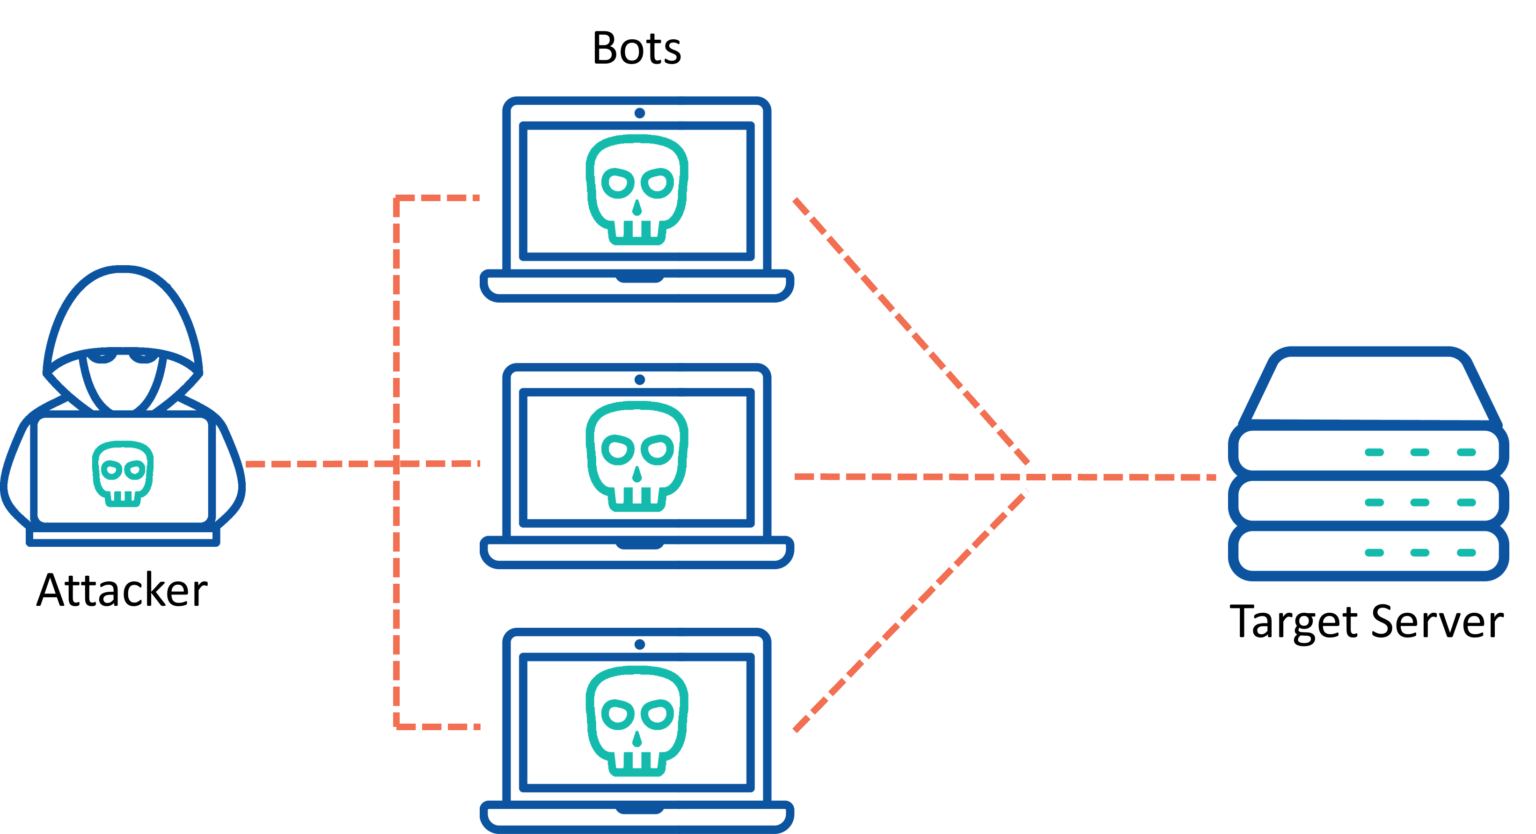
\includegraphics[width=0.6\textwidth]{ataqueDDoS.png}
        \caption{Arquitetura de um ataque DDoS}
        \legend{Fonte: \citeonline{Apposite2025}}
    \end{figure}

    \FloatBarrier


\subsection{Análise do Dataset CICDDoS2019}
O conjunto de dados CICDDoS2019, desenvolvido pelo Canadian Institute for Cybersecurity (CIC) da University of New Brunswick, foi criado com o objetivo de fornecer uma base moderna e realista para pesquisas relacionadas à detecção de ataques distribuídos de negação de serviço (DDoS) utilizando técnicas de aprendizado de máquina e mineração de dados. Esse dataset foi projetado para representar cenários atuais de tráfego de rede, combinando atividades benignas com múltiplos tipos de ataques DDoS, permitindo a avaliação mais precisa de modelos de detecção de intrusão.


O CICDDoS2019 disponibiliza os dados nos formatos PCAP, que contém o tráfego bruto da rede, e CSV, com mais de 80 atributos extraídos dos fluxos de comunicação, o que facilita sua utilização em modelos de aprendizado de máquina e análises estatísticas. O dataset foi desenvolvido em um ambiente experimental controlado, composto por diferentes sistemas operacionais, servidores e dispositivos de segurança, com o objetivo de simular cenários reais de redes corporativas. Dessa forma, o CICDDoS2019 constitui uma base relevante para o treinamento e validação de modelos de detecção de intrusão, permitindo a identificação de padrões associados a ataques DDoS e contribuindo para o desenvolvimento de soluções mais eficazes para a segurança de redes \cite{Sharafaldin2019}. 

A Figura 4 apresenta a distribuição percentual dos diferentes tipos de tráfego presentes no conjunto de dados CICDDoS2019. Observa-se que o dataset é composto por tráfego legítimo e múltiplas categorias de ataques DDoS, refletindo um cenário mais próximo de ambientes reais de rede. Essa diversidade de classes contribui para a avaliação de modelos de aprendizado de máquina em diferentes padrões de tráfego, permitindo analisar sua capacidade de distinguir atividades normais de comportamentos maliciosos associados a ataques distribuídos de negação de serviço

\begin{figure}[h]
    \centering
    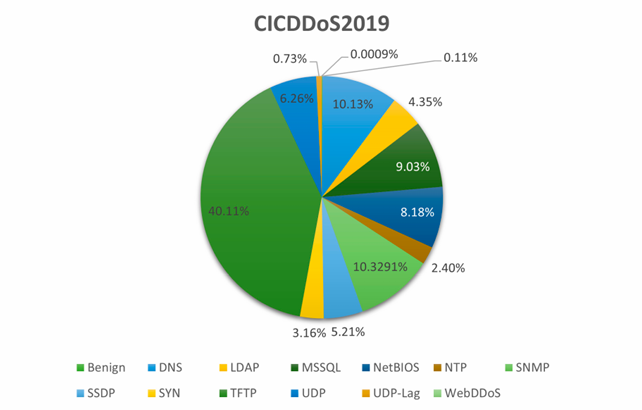
\includegraphics[width=0.90\textwidth]{dataset.png}
    \caption{Porcentagem de classes do dataset - CICDDoS2019}
    \legend{Fonte: \citeonline{Elubeyd2023}}
\end{figure}

\FloatBarrier

\subsection{Inteligência Artificial}
Nos fundamentos da obra de \citeonline{Russell2010}, a Inteligência Artificial (IA) pode ser compreendida como o campo da ciência da computação dedicado ao desenvolvimento de sistemas capazes de simular capacidades cognitivas humanas, como raciocínio, aprendizagem, percepção, tomada de decisão e resolução de problemas. Segundo \citeonline{Russell2010}, a IA envolve a criação de agentes inteligentes capazes de perceber o ambiente em que estão inseridos e agir de maneira racional para atingir objetivos específicos. Entre suas principais aplicações estão a automação de processos, reconhecimento de padrões, processamento de linguagem natural e análise preditiva, sendo seu uso cada vez mais relevante em áreas como segurança da informação e detecção de intrusões. Nesse contexto, técnicas de aprendizado de máquina, um dos principais ramos da IA, permitem que sistemas identifiquem comportamentos anômalos em grandes volumes de dados, contribuindo para a detecção mais rápida e precisa de ameaças cibernéticas \cite{Russell2010}. 

\subsection{Machine Learning}
Como uma das principais áreas derivadas da Inteligência Artificial (IA), o Machine Learning (ML) surge como uma abordagem voltada ao desenvolvimento de sistemas capazes de aprender a partir de dados e aprimorar seu desempenho de forma progressiva, sem depender exclusivamente de regras previamente programadas \cite{Russell2010,Mitchell1997}.
De acordo com \citeonline{Russell2010}, a capacidade de adaptação e aprendizado constitui um dos elementos centrais para a construção de agentes inteligentes, tornando o aprendizado automatizado um componente fundamental da evolução da IA. Nesse contexto, o aprendizado de máquina permite que modelos computacionais identifiquem padrões, realizem previsões e apoiem processos de tomada de decisão em cenários complexos.
Segundo \citeonline{Mitchell1997}, o aprendizado de máquina baseia-se no desenvolvimento de algoritmos capazes de melhorar seu desempenho a partir da experiência obtida por meio dos dados. Dessa forma, o ML utiliza métodos estatísticos e computacionais para extrair conhecimento de grandes volumes de informações, sendo amplamente aplicado em problemas que exigem análise contínua, identificação de padrões e apoio à tomada de decisão.
Além disso, essa área abrange diferentes tipos de aprendizado, que variam de acordo com a natureza dos dados e com os objetivos específicos de cada aplicação, sendo seu entendimento essencial para a utilização dessas técnicas em sistemas de detecção de intrusão e resposta a ameaças cibernéticas \cite{Mitchell1997,Russell2010}. 


\subsection{Machine Learning aplicado à detecção de intrusão}
A aplicação de Machine Learning (ML) em sistemas de detecção de intrusão tem se consolidado como uma abordagem estratégica para aprimorar a identificação de ameaças em ambientes computacionais, especialmente diante do aumento da complexidade e do volume do tráfego de rede \cite{Gopalakrishnan2023}. 


Diferentemente dos métodos tradicionais baseados em assinaturas, os modelos de aprendizado de máquina permitem analisar grandes volumes de dados e identificar padrões associados a comportamentos normais e anômalos, possibilitando a detecção de ataques previamente desconhecidos e maior capacidade de adaptação a novas ameaças \cite{Gopalakrishnan2023}. Nesse contexto, o ML é empregado na extração e análise de características do tráfego de rede, permitindo a classificação automática de eventos e contribuindo para a melhoria da precisão dos sistemas de detecção de intrusão \cite{Gopalakrishnan2023}. 


Entre suas aplicações específicas, destaca-se a detecção de ataques de Distributed Denial of Service (DDoS). Dessa forma, a aplicação de ML à detecção de intrusão representa um avanço importante para a segurança cibernética, contribuindo para o desenvolvimento de sistemas mais inteligentes, resilientes e capazes de responder de forma mais eficaz às ameaças emergentes \cite{Gopalakrishnan2023,Aktar2023}. 

\subsection{Algoritmos de Aprendizado de Máquina}
Segundo \citeonline{Russell2010}, o aprendizado ocorre a partir de diferentes tipos de feedback recebidos pelo agente, esses feedbacks determinam as principais categorias de algoritmos de aprendizado de máquina.


De forma geral, o processo de aprendizado de máquina envolve a utilização de conjuntos de dados para treinar modelos computacionais capazes de reconhecer padrões e realizar previsões. Conforme apresentado por \citeonline{Gopalakrishnan2023}, esse processo é composto principalmente por duas etapas: treinamento do modelo e teste ou tomada de decisão. Durante o treinamento, os dados passam por etapas de pré-processamento e extração de características, permitindo que o modelo aprenda padrões presentes nos dados. Posteriormente, o modelo treinado é utilizado para analisar novos dados, chamados de dados de teste, possibilitando também a avaliação de sua precisão\cite{Gopalakrishnan2023}.


Os algoritmos de aprendizado de máquina podem ser classificados em três principais categorias: aprendizado supervisionado, aprendizado não supervisionado e aprendizado por reforço. Essa divisão ocorre de acordo com a forma como o sistema recebe informações e aprende durante o processo de treinamento \cite{Gopalakrishnan2023}.


O aprendizado supervisionado caracteriza-se pela utilização de exemplos rotulados, ou seja, dados de entrada associados às respectivas saídas esperadas. Entre os principais algoritmos supervisionados destacam-se o Support Vector Machine (SVM) e o Random Forest \cite{Russell2010, Gopalakrishnan2023}. 


O aprendizado não supervisionado diferencia-se por não utilizar dados rotulados durante o treinamento. Nesse caso, o objetivo do algoritmo é identificar padrões, agrupamentos ou relações existentes nos dados sem conhecimento prévio das respostas corretas. \citeonline{Russell2010} afirmam que esse tipo de aprendizado permite ao agente detectar agrupamentos potencialmente úteis em conjuntos de dados, sendo o agrupamento (clustering) uma das tarefas mais comuns dessa categoria. Como exemplos de um algoritmo não supervisionado, pode ser citado o K-Means \cite{Gopalakrishnan2023}.


Por sua vez, o aprendizado por reforço baseia-se em um sistema de recompensas e punições, no qual o agente aprende por tentativa e erro ao interagir com o ambiente. De acordo com \citeonline{Russell2010}, o agente recebe reforços positivos ou negativos conforme suas ações, ajustando seu comportamento para maximizar recompensas futuras. O algoritmo Q-Learning pode ser citado como um exemplo dessa abordagem \cite{Russell2010}.

\subsection{Aprendizado Supervisionado}
O aprendizado supervisionado é um dos paradigmas mais tradicionais e amplamente utilizados no campo do aprendizado de máquina, sendo aplicado principalmente em problemas de classificação, regressão e ranqueamento. Nesse modelo, o algoritmo recebe um conjunto de dados previamente rotulados, denominado conjunto de treinamento, e utiliza essas informações para aprender padrões capazes de realizar previsões sobre dados ainda não observados \cite{Mohri2018}.


Segundo \citeonline{Mohri2018}, o aprendizado supervisionado consiste em fornecer ao aprendiz exemplos rotulados para que ele consiga fazer previsões em pontos desconhecidos, sendo esse o cenário mais comum em aplicações de machine learning.


De acordo com \citeonline{Luxburg2008}, o problema mais estudado dentro do aprendizado de máquina é a classificação supervisionada. Nesse cenário, existem dois conjuntos fundamentais: o espaço de entrada, representado por X, que contém as instâncias ou objetos, e o espaço de saída, representado por Y, correspondente aos rótulos ou categorias possíveis. O processo de aprendizagem ocorre a partir de pares ordenados compostos por uma entrada e sua respectiva saída correta: (X1,Y1),...,(Xn,Yn), permitindo ao algoritmo identificar uma relação funcional entre os dados de entrada e os rótulos desejados \cite{Luxburg2008}.


O objetivo do aprendizado supervisionado é encontrar uma função de mapeamento f:X→Y. Essa função, denominada classificador, deve atribuir corretamente os rótulos às instâncias analisadas. Para isso, o algoritmo recebe um conjunto de treinamento formado por exemplos rotulados e, a partir deles, produz um modelo capaz de inferir resultados para novos dados \cite{Luxburg2008}.


Segundo \citeonline{Luxburg2008}, o aprendizado supervisionado recebe esse nome porque o algoritmo possui acesso às respostas corretas durante o treinamento. Dessa forma, o sistema consegue avaliar continuamente se suas previsões estão corretas, caracterizando um processo de aprendizagem guiado ou supervisionado. Em problemas de classificação binária, por exemplo, os rótulos geralmente pertencem ao conjunto {-1, +1}, indicando duas possíveis categorias para cada objeto analisado \cite{Luxburg2008}.

\subsection{Decision Trees}
As \textit{árvores de decisão} (Decision Trees – DT) são modelos de aprendizado supervisionado amplamente utilizados em tarefas de classificação e regressão devido à sua simplicidade, interpretabilidade e eficiência computacional. Segundo \citeonline{Breiman1984}, as árvores de decisão possuem uma estrutura hierárquica composta por nós, ramos e folhas. Os nós representam pontos de decisão nos quais determinados atributos dos dados são avaliados; os ramos representam os possíveis caminhos resultantes dessas decisões; e as folhas correspondem às classes ou valores finais previstos pelo modelo.
O funcionamento de uma árvore de decisão ocorre por meio de divisões sucessivas do conjunto de dados. Durante o treinamento, o algoritmo seleciona os atributos mais relevantes para separar os dados em subconjuntos cada vez mais homogêneos. Esse processo é realizado de forma recursiva até que critérios de parada sejam atingidos, como profundidade máxima da árvore ou quantidade mínima de instâncias em um nó. De acordo com \citeonline{Breiman1984}, o objetivo dessas divisões é reduzir a impureza dos grupos formados, permitindo que o modelo identifique padrões presentes nos dados de treinamento.
Os nós da árvore representam pontos em que uma decisão é tomada com base em uma característica específica do conjunto de dados. Dependendo do valor do atributo analisado, o fluxo segue por diferentes ramos até alcançar uma folha, responsável pela previsão final do modelo. Essa estrutura torna as árvores de decisão facilmente interpretáveis, permitindo compreender de maneira clara como as previsões são realizadas.
Apesar das vantagens relacionadas à simplicidade e interpretabilidade, árvores de decisão individuais podem apresentar elevada sensibilidade aos dados de treinamento. Isso ocorre porque o modelo pode aprender excessivamente os detalhes e ruídos presentes no conjunto de treinamento, fenômeno conhecido como overfitting. O overfitting reduz a capacidade de generalização do algoritmo, fazendo com que o modelo apresente bom desempenho nos dados utilizados no treinamento, mas baixa precisão ao lidar com novos exemplos \cite{Breiman1984}.

\subsection{Random Forest}
O algoritmo \textit{Random Forest} é um dos métodos de aprendizado supervisionado mais utilizados na área de machine learning, especialmente em problemas de classificação e regressão. Proposto por Leo Breiman em 2001, o modelo pertence à categoria de métodos conhecidos como ensemble learning, cuja principal característica é a combinação de múltiplos modelos para produzir resultados mais precisos, robustos e com maior capacidade de generalização \cite{Breiman2001}.
O Random Forest utiliza múltiplas árvores de decisão independentes como base para seu funcionamento. Em vez de utilizar apenas uma única árvore para realizar previsões, o algoritmo cria uma “floresta” composta por diversas árvores treinadas separadamente. Essa abordagem reduz os problemas de variância e overfitting encontrados em árvores individuais, aumentando a robustez e a estabilidade do modelo \cite{Breiman2001}.
Durante o treinamento, cada árvore é construída a partir de subconjuntos aleatórios do conjunto de dados original utilizando a técnica denominada bootstrap sampling. Essa técnica consiste em gerar várias amostras aleatórias com reposição a partir do conjunto de treinamento. Dessa forma, algumas instâncias podem ser repetidas enquanto outras podem não ser selecionadas em determinada amostra. Como consequência, cada árvore é treinada com dados ligeiramente diferentes, aumentando a diversidade entre os modelos da floresta.
Além disso, durante o processo de construção das árvores, o algoritmo considera apenas subconjuntos aleatórios de atributos para realizar as divisões dos nós. Segundo \citeonline{Breiman2001}, essa aleatoriedade reduz a correlação entre as árvores individuais, contribuindo para melhorar a capacidade de generalização do modelo e reduzir erros de previsão.
No processo de classificação, cada árvore da floresta realiza uma previsão individual para a instância analisada. O resultado final é definido por meio de votação majoritária, na qual a classe mais frequentemente prevista entre as árvores é escolhida como resposta final. Em problemas de regressão, o resultado geralmente corresponde à média dos valores previstos pelas árvores individuais. Essa estratégia reduz significativamente os efeitos do overfitting e melhora a estabilidade das previsões realizadas pelo modelo \cite{Breiman2001}.
Outra característica importante do Random Forest é sua capacidade de lidar com grandes volumes de dados e conjuntos com alta dimensionalidade. O algoritmo também possibilita medir a importância das variáveis utilizadas durante o treinamento, permitindo identificar quais atributos exercem maior influência nas previsões realizadas. Além disso, apresenta elevada tolerância a ruídos, dados ausentes e variações nos conjuntos de treinamento, fatores que contribuíram para sua ampla utilização em áreas como análise preditiva, reconhecimento de padrões, detecção de fraudes, mineração de dados e sistemas inteligentes \cite{Breiman2001}.
Dessa forma, o Random Forest pode ser compreendido como uma evolução das árvores de decisão tradicionais, utilizando a combinação de múltiplas árvores independentes para reduzir erros de generalização e aumentar a precisão das previsões. A utilização conjunta de diferentes árvores permite que o modelo apresente desempenho superior ao de árvores isoladas, consolidando o Random Forest como um dos algoritmos mais eficientes e populares do aprendizado de máquina contemporâneo.

\subsection{Support Vector Machine}
O algoritmo \textit{Support Vector Machine} (SVM) é um método de aprendizado supervisionado amplamente utilizado em problemas de classificação e regressão, sendo reconhecido por sua elevada capacidade de generalização e eficiência em conjuntos de dados de alta dimensionalidade. O modelo foi formalizado por Corinna Cortes e Vladimir Vapnik em 1995, fundamentando-se nos princípios da Teoria do Aprendizado Estatístico (Statistical Learning Theory), desenvolvida por \citeonline{Vapnik1998}. O principal objetivo do SVM é encontrar uma fronteira de decisão capaz de separar diferentes classes de dados da forma mais otimizada possível \cite{Cortes1995}.
O funcionamento do SVM baseia-se na construção de um hiperplano de separação entre classes. Em problemas bidimensionais, esse hiperplano pode ser compreendido como uma linha que divide os dados em diferentes categorias; em espaços multidimensionais, corresponde a uma superfície de separação. Segundo \citeonline{Cortes1995}, o algoritmo busca identificar o hiperplano que maximize a distância entre as classes, denominada margem (margin). Quanto maior essa margem, maior tende a ser a capacidade de generalização do modelo para novos dados.
Os elementos mais importantes para a definição do hiperplano são chamados de vetores de suporte (support vectors). Esses vetores correspondem às instâncias de treinamento localizadas mais próximas da fronteira de separação. Dessa forma, são os pontos que efetivamente influenciam a posição e orientação do hiperplano. De acordo com \citeonline{Vapnik1998}, a utilização apenas dos vetores de suporte torna o modelo eficiente e reduz a complexidade do processo de classificação.
Em situações nas quais os dados não podem ser separados linearmente, o SVM utiliza funções conhecidas como kernels. Os kernels permitem transformar os dados originais para espaços de maior dimensionalidade, tornando possível encontrar uma separação linear em um novo espaço de representação. Entre os principais tipos de kernel utilizados estão o linear, polinomial e radial (Radial Basis Function – RBF). Conforme descrito por \citeonline{Cortes1995}, essa abordagem possibilita ao SVM lidar com problemas complexos e não linearmente separáveis.
A Teoria do Aprendizado Estatístico, proposta por \citeonline{Vapnik1998}, fornece a base teórica para o funcionamento do SVM. Segundo essa teoria, o objetivo de um modelo de aprendizado não é apenas minimizar erros no conjunto de treinamento, mas também maximizar sua capacidade de generalização para dados não observados. Nesse contexto, o SVM busca equilibrar a complexidade do modelo e o desempenho obtido durante o treinamento, reduzindo problemas de overfitting.

O SVM reduz esse problema por meio da maximização da margem entre as classes, estratégia que favorece modelos mais robustos e menos sensíveis às variações dos dados \cite{Vapnik1998}.
Outra característica importante do SVM é sua eficiência em conjuntos de dados com grande quantidade de atributos. O algoritmo apresenta bom desempenho em aplicações envolvendo reconhecimento de padrões, classificação de textos, bioinformática, detecção de fraudes, visão computacional e processamento de linguagem natural. Além disso, mesmo em cenários com poucos exemplos de treinamento, o modelo pode apresentar elevada precisão devido à sua forte fundamentação matemática \cite{Cortes1995}.
Embora seja tradicionalmente utilizado em problemas de classificação binária, o SVM também pode ser adaptado para classificação multiclasse e tarefas de regressão. No caso da regressão, utiliza-se uma variação denominada Support Vector Regression (SVR), que busca encontrar uma função capaz de aproximar os dados com o menor erro possível, mantendo as propriedades de generalização do modelo.
Dessa forma, o Support Vector Machine consolidou-se como um dos algoritmos mais importantes do aprendizado de máquina moderno, combinando sólida fundamentação teórica com elevada eficiência prática. Sua capacidade de maximizar a margem de separação, lidar com dados não lineares por meio de kernels e reduzir problemas de overfitting contribuiu para sua ampla utilização em diferentes áreas da inteligência artificial e análise de dados.


\subsection{Métricas de Avaliação de Modelos}
\subsection{Acurácia}
A acurácia é uma das métricas mais utilizadas para avaliar modelos de classificação em aprendizado de máquina. Essa métrica representa a proporção total de previsões corretas realizadas pelo modelo em relação ao número total de instâncias analisadas. Segundo \citeonline{Rainio2024}, a acurácia expressa o percentual de classificações corretas considerando tanto os exemplos positivos quanto os negativos.
Em problemas de classificação binária, cada previsão realizada pelo modelo pode ser categorizada em quatro tipos principais: verdadeiro positivo (True Positive – TP), verdadeiro negativo (True Negative – TN), falso positivo (False Positive – FP) e falso negativo (False Negative – FN). Um verdadeiro positivo ocorre quando uma instância positiva é corretamente classificada como positiva; um verdadeiro negativo corresponde a uma instância negativa corretamente classificada como negativa; um falso positivo ocorre quando uma instância negativa é incorretamente classificada como positiva; e um falso negativo ocorre quando uma instância positiva é incorretamente classificada como negativa \cite{Rainio2024}.
A fórmula da acurácia é dada por:

\begin{equation}
Accuracy = \frac{TP + TN}{TP + TN + FP + FN}
\end{equation}


Onde:
TP (True Positive): quantidade de verdadeiros positivos;
TN (True Negative): quantidade de verdadeiros negativos;
FP (False Positive): quantidade de falsos positivos;
FN (False Negative): quantidade de falsos negativos.
O valor da acurácia pertence ao intervalo [0,1], no qual valores mais próximos de 1 indicam melhor desempenho do modelo. Entretanto, conforme destacado por \citeonline{Rainio2024}, a acurácia pode não ser suficiente para avaliar modelos em conjuntos de dados desbalanceados, isto é, quando existe grande diferença entre a quantidade de exemplos positivos e negativos. Nesses casos, métricas como recall tornam-se mais adequadas para analisar o comportamento do modelo.

\subsection{Recall}
O recall (revocação) ou taxa de verdadeiros positivos, é uma métrica utilizada para medir a capacidade do modelo de identificar corretamente as instâncias positivas. Segundo \citeonline{Rainio2024}, o recall representa a proporção de exemplos positivos que foram corretamente classificados pelo algoritmo.
Essa métrica é especialmente importante em aplicações nas quais identificar corretamente os casos positivos é essencial, como diagnósticos médicos, detecção de fraudes e sistemas de segurança. Em tais cenários, falsos negativos podem causar impactos significativos, tornando necessário maximizar a taxa de identificação correta dos exemplos positivos.
A fórmula do recall é dada por:

\begin{equation}
Recall = \frac{TP}{TP + FN}
\end{equation}

O valor do recall também pertence ao intervalo [0,1], sendo que valores próximos de 1 indicam que o modelo consegue identificar corretamente a maior parte das instâncias positivas presentes no conjunto de dados. Conforme discutido por \citeonline{Rainio2024}, métricas como recall frequentemente fornecem informações mais relevantes do que a acurácia em problemas com classes desbalanceadas, pois avaliam separadamente o desempenho do modelo em relação às classes positivas e negativas.

\subsection{Precisão}
A precisão é uma métrica que indica a proporção de instâncias classificadas como positivas que foram corretamente identificadas pelo modelo, sendo calculada pela razão entre os verdadeiros positivos (TP) e o total de predições positivas (TP + FP). Embora o par precisão/revocação forneça insights úteis sobre o comportamento de um classificador, \citeonline{Chicco2020} ressaltam que a precisão e o F1-score (sua média harmônica com a revocação) podem apresentar resultados "perigosamente otimistas" e inflados, especialmente em conjuntos de dados desbalanceados. Isso ocorre porque essas métricas são independentes do número de amostras corretamente classificadas como negativas (TN). Por essa razão, os autores argumentam que, para uma avaliação mais informativa e fiel em tarefas de classificação binária, deve-se preferir o Coeficiente de Correlação de Matthews (MCC), que integra as quatro categorias da matriz de confusão e produz um escore alto apenas se o modelo obtiver bons resultados tanto na classe positiva quanto na negativa. 
A fórmula da precisão é dada por:

\begin{equation}
\text{Precisão} = \frac{TP}{TP + FP}
\end{equation}

\subsection{F1-Score}
O F1-score é uma métrica amplamente utilizada para avaliar o desempenho de modelos de classificação, especialmente em cenários com desequilíbrio entre as classes \cite{Hand2021}. Essa métrica corresponde à média harmônica entre a precisão e a revocação, permitindo combinar dois aspectos distintos e complementares do desempenho do modelo \cite{Hand2021}. Diferentemente de medidas que podem ser infladas por grandes volumes de casos negativos, o F1-score foca nos casos positivos de interesse, sendo particularmente relevante em domínios onde os verdadeiros negativos não são a prioridade, como na detecção de fraudes e em problemas de classificação em disciplinas computacionais \cite{Hand2021}. 
Essa métrica corresponde à média harmônica entre a precisão e a revocação, sendo calculada pela fórmula: F1 = 2 × (Precisão × Revocação) / (Precisão + Revocação).
A fórmula do f1-score é dada por:

\begin{equation}
F1 = 2 \cdot \frac{\text{Precisão} \cdot \text{Revocação}}{\text{Precisão} + \text{Revocação}}
\end{equation}

A precisão representa a proporção de instâncias classificadas como positivas que estão corretas, enquanto a revocação indica a capacidade do modelo de identificar corretamente todos os casos positivos presentes no conjunto de dados.

\subsection{Coeficiente de correlação de Matthews (MCC)}
é uma métrica utilizada para avaliar o desempenho de classificadores binários, sendo especialmente adequada para conjuntos de dados desbalanceados. Diferentemente da acurácia, o MCC considera simultaneamente os valores de verdadeiros positivos, verdadeiros negativos, falsos positivos e falsos negativos, fornecendo uma avaliação mais equilibrada do modelo. Seus valores variam entre -1 e 1, em que 1 representa uma classificação perfeita, 0 indica desempenho equivalente ao acaso e valores negativos refletem predições inconsistentes em relação aos valores reais. Por considerar todos os elementos da matriz de confusão, o MCC é frequentemente recomendado como uma métrica robusta para a avaliação de modelos de aprendizado de máquina em problemas de classificação binária \cite{Chicco2023}. 
A fórmula é do MCC dada por:

\begin{equation}
MCC = \frac{(TP \times TN) - (FP \times FN)}
{\sqrt{(TP + FP)(TP + FN)(TN + FP)(TN + FN)}}
\label{eq:mcc}
\end{equation}



% ---------------------------------------------------------------

% % ---------------------------------------------------------------
% \section{Fundamentos}
% \label{sec:fundamentos}

% Este trabalho utiliza conceitos de aprendizado de máquina supervisionado aplicados à detecção de intrusão.

% O algoritmo Random Forest é baseado em múltiplas árvores de decisão e realiza classificações combinando os resultados dessas árvores, aumentando a precisão e reduzindo overfitting.

% O Support Vector Machine (SVM) busca encontrar um hiperplano que melhor separa as classes de dados, sendo eficiente em problemas com alta dimensionalidade.

% O Multi-Layer Perceptron (MLP) é uma rede neural artificial composta por múltiplas camadas, capaz de aprender padrões complexos por meio de treinamento supervisionado.

% Para avaliação dos modelos, serão utilizadas as métricas:

% \begin{itemize}
%     \item Acurácia
%     \item Precisão
%     \item Recall
%     \item F1-Score
% \end{itemize}

% Essas métricas permitem avaliar o desempenho dos algoritmos de forma mais completa, especialmente em cenários com dados desbalanceados.

% % ---------------------------------------------------------------
\section{Trabalhos relacionados}
\label{sec:trabalhos_relacionados}

\subsection{Trabalho 1: An Analysis of Intrusion Detection Classification using Supervised Machine Learning Algorithms on NSL-KDD Dataset}

\citeonline{Rastogi2022} investigaram o uso de algoritmos supervisionados de aprendizado de máquina para classificação de intrusões em redes, com foco na melhoria da precisão de sistemas IDS baseados em anomalias. Os autores compararam diferentes algoritmos, incluindo Support Vector Machine (SVM), Random Forest (RF), K-Nearest Neighbors (KNN), Naive Bayes, Decision Tree e Logistic Regression, utilizando o conjunto de dados NSL-KDD para classificação binária e multiclasse. Os resultados demonstraram que o Random Forest apresentou um dos melhores desempenhos em termos de acurácia e tempo de execução, enquanto o SVM obteve desempenho satisfatório, porém com maior custo computacional.

O presente trabalho diferencia-se por utilizar o conjunto CICDDoS2019, mais recente e específico para ataques DDoS, além de concentrar a análise comparativa exclusivamente nos algoritmos Random Forest e Support Vector Machine, buscando avaliar qual modelo apresenta melhor desempenho preditivo na detecção desse tipo específico de ameaça.


\subsection{Trabalho 2: Detecting DDoS Threats Using Supervised Machine Learning for Traffic Classification in Software Defined Networking}

\citeonline{Hirsi2024} abordaram a detecção de ataques DDoS em ambientes de Software-Defined Networking (SDN) por meio de técnicas supervisionadas de aprendizado de máquina para classificação de tráfego. O estudo propôs uma abordagem baseada em classificação binária entre tráfego benigno e malicioso, utilizando um conjunto de dados próprio validado com o CICDDoS2019. Entre os algoritmos avaliados, o Random Forest apresentou o melhor resultado, alcançando 98,97\% de acurácia e baixa taxa de falso alarme, demonstrando elevada eficiência para identificação de ameaças em tempo real.

Diferentemente desse estudo, que enfatiza um cenário específico de redes SDN e prioriza o modelo de melhor desempenho, o presente trabalho propõe uma comparação direta entre Random Forest e Support Vector Machine em um contexto mais geral de sistemas IDS baseados em anomalias, buscando identificar qual algoritmo oferece melhor equilíbrio entre desempenho e aplicabilidade na detecção de ataques DDoS.


\subsection{Trabalho 3: Distributed Denial-of-Service (DDoS) Attack Detection Using Supervised Machine Learning Algorithms}

\citeonline{Abiramasundari2025} propuseram um modelo de detecção de ataques DDoS baseado em aprendizado supervisionado, denominado PCA-based Enhanced Distributed DDoS Attack Detection (EDAD). O estudo utilizou técnicas de pré-processamento, normalização, balanceamento de classes e redução de dimensionalidade por Principal Component Analysis (PCA), além de comparar diversos algoritmos, como SVM, Random Forest, Decision Tree, KNN e Logistic Regression, em diferentes bases de dados, incluindo o CICDDoS2019. Os resultados indicaram que o Random Forest e o KNN obtiveram os melhores desempenhos no CICDDoS2019, com acurácia de 98,7\%.

O presente trabalho diferencia-se por restringir a análise aos algoritmos Random Forest e Support Vector Machine, permitindo uma comparação mais aprofundada entre dois modelos amplamente utilizados na literatura. Além disso, o foco está na avaliação detalhada das métricas de acurácia, precisão, recall, F1-score e MCC visando identificar a abordagem mais eficiente para classificação binária entre tráfego normal e anômalo.

\vspace{0.5cm}

\begin{table}[htb]
    \centering
    \caption{Comparação entre trabalhos relacionados}
    \label{tab:trabalhos_relacionados}
    
    \renewcommand{\arraystretch}{1.3}
    
    \begin{tabularx}{\textwidth}{p{3cm}|X|X|X|X}
        \toprule
        \textbf{Critério} & \textbf{Trabalho 1} & \textbf{Trabalho 2} & \textbf{Trabalho 3} & \textbf{Este trabalho} \\
        \midrule
        
        \textbf{Objetivo}           
        & Avaliar algoritmos supervisionados para detecção de intrusões no NSL-KDD
        & Detectar ataques DDoS em ambiente SDN com aprendizado supervisionado
        & Propor e avaliar detecção de DDoS com PCA e modelos supervisionados
        & Comparar Random Forest e SVM na detecção de DDoS em IDS
        \\
        \midrule
        
        \textbf{Tecnologias}         
        & SVM, Random Forest, KNN, Naive Bayes, Decision Tree, Logistic Regression
        & Random Forest, SVM e outros classificadores supervisionados
        & SVM, Random Forest, Decision Tree, KNN, Logistic Regression + PCA
        & Random Forest e SVM
        \\
        \midrule
        
        \textbf{Base de dados}          
        & NSL-KDD
        & CICDDoS2019 (validado em cenário SDN)
        & CICDDoS2019 e outras bases de DDoS
        & CICDDoS2019
        \\
        \midrule
        
        \textbf{Validação}          
        & Avaliação comparativa com métricas de acurácia e tempo de execução
        & Avaliação de acurácia e taxa de falso positivo em SDN
        & Uso de PCA + avaliação comparativa de modelos supervisionados
        & Avaliação com acurácia, precisão, recall, F1-score e MCC
        \\
        \midrule
        
        \textbf{Resultados principais}          
        & Random Forest apresentou melhor desempenho geral
        & Random Forest obteve alta acurácia ($\approx 98{,}97\%$)
        & Random Forest e KNN apresentaram melhor desempenho ($\approx 98{,}7\%$)
        & Identificar o melhor equilíbrio entre SVM e Random Forest
        \\
        \midrule
        
        \textbf{Limitações}          
        & Pouca diversidade de modelos
        & Foco específico em ambiente SDN
        & Uso de PCA e pipeline mais complexo
        & ---
        \\
        
        \bottomrule
    \end{tabularx}
    
    \legend{Fonte: Elaborado pelo autor (2026)}
\end{table}

% ===============================================================
% CAPÍTULO 3 - DESENVOLVIMENTO
% ===============================================================
\chapter{Desenvolvimento}
\label{cap:desenvolvimento}

% ---------------------------------------------------------------
\section{Solução proposta}
\label{sec:solucao}

\subsection{Visão geral da solução} A solução proposta neste trabalho consiste na análise e comparação entre dois algoritmos de aprendizado de máquina supervisionado, Support Vector Machine (SVM) e Random Forest (RF), aplicados ao problema de detecção de ataques DDoS em redes de computadores. O objetivo central é avaliar o desempenho desses modelos na tarefa de classificação binária, distinguindo tráfego normal de tráfego malicioso, contribuindo para o fortalecimento de sistemas de detecção de intrusão (IDS). Essa abordagem se baseia no uso de técnicas de machine learning amplamente empregadas em problemas de cibersegurança, onde a identificação de padrões em grandes volumes de dados de rede permite detectar comportamentos anômalos com maior eficiência. Dessa forma, a solução busca não apenas aplicar os modelos, mas também realizar uma análise comparativa de sua eficácia no contexto de ataques DDoS.

\subsection{Metodologia} A metodologia da solução foi estruturada em etapas sequenciais, organizadas em uma construção de processamento de dados e treinamento de modelos. Inicialmente, foi realizado um levantamento bibliográfico com o objetivo de compreender os principais conceitos relacionados a ataques DDoS, sistemas IDS e algoritmos de aprendizado supervisionado aplicados à segurança de redes.

Na segunda etapa, será analisado o conjunto de dados CICDDoS2019. \citeonline{Salih2024} destaca que o CICDDoS2019 se tornou uma das principais bases utilizadas em pesquisas de segurança computacional devido à diversidade de ataques presentes e à grande quantidade de fluxos de rede disponíveis para treinamento e validação de modelos supervisionados. 

O CICDDoS2019 possui mais de 50 milhões de registros de tráfego malicioso e mais de 100 mil registros benignos, organizados em arquivos CSV e PCAP que totalizam mais de 20 GB de dados. O dataset contém 13 classes principais, sendo uma classe BENIGN, correspondente ao tráfego legítimo da rede, e 12 categorias de ataques DDoS. Os ataques presentes no CICDDoS2019 são: DrDoS\_DNS, DrDoS\_LDAP, DrDoS\_MSSQL, DrDoS\_NTP, DrDoS\_NetBIOS, DrDoS\_SNMP, DrDoS\_SSDP, DrDoS\_UDP, Syn, TFTP, UDP-Lag e WebDDoS. Essas classes representam diferentes técnicas de ataques distribuídos de negação de serviço, permitindo que os modelos supervisionados sejam treinados para identificar múltiplos padrões de comportamento malicioso em tráfego de rede \cite{Salih2024}. Já os atributos (features) representam as características numéricas e estatísticas extraídas de cada fluxo de rede, O CICDDoS2019 disponibiliza aproximadamente 87 atributos, utilizados pelos algoritmos para identificar padrões de comportamento malicioso \cite{Salih2024}. 

Esses atributos descrevem estatisticamente o comportamento do fluxo de rede e são utilizados pelos modelos de aprendizado supervisionado durante a etapa de treinamento. Entre as principais features presentes no dataset destacam-se Flow Duration, que representa o tempo total de duração do fluxo; Total Fwd Packets e Total Backward Packets, responsáveis por indicar a quantidade de pacotes enviados e recebidos; Flow Bytes/s e Flow Packets/s, que representam a taxa de transferência de bytes e pacotes por segundo; Packet Length Mean, relacionada ao tamanho médio dos pacotes transmitidos; além da feature SYN Flag Count, que contabiliza a quantidade de pacotes TCP SYN presentes na comunicação \cite{Salih2024}. 

Pesquisas recentes apontam que atributos relacionados à taxa de pacotes, duração do fluxo, quantidade de bytes transmitidos e flags TCP estão entre as features mais relevantes para o reconhecimento de ataques DDoS baseados em flooding, especialmente SYN Flood, UDP Flood, LDAP Amplification e DNS Amplification \cite{Salih2024}. Em ataques SYN Flood, por exemplo, a feature SYN Flag Count tende a apresentar valores extremamente elevados devido ao grande volume de requisições SYN enviadas ao servidor alvo. Já em ataques UDP Flood e LDAP Amplification, atributos como Flow Packets/s, Flow Bytes/s e Packet Length Mean tornam-se relevantes devido ao aumento anormal do tráfego e da taxa de transmissão de pacotes \cite{Salih2024}. 

Considerando o elevado volume de dados presente no CICDDoS2019, que possui milhões de registros de tráfego de rede, será realizado um recorte controlado do conjunto de dados por meio de técnicas de amostragem, visando tornar o processamento viável no ambiente Jupyter Notebook e reduzir o custo computacional associado ao treinamento dos modelos, especialmente do Support Vector Machine, cuja complexidade computacional tende a aumentar significativamente em grandes conjuntos de dados.

Apesar de sua ampla utilização acadêmica, o CICDDoS2019 apresenta limitações que podem introduzir vieses nos modelos de aprendizado de máquina. Um dos principais problemas identificados na literatura é o forte desbalanceamento entre as classes, uma vez que determinados ataques possuem milhões de registros enquanto outros apresentam poucas centenas de amostras. Esse cenário pode levar os algoritmos a favorecerem classes majoritárias durante o treinamento, reduzindo a capacidade de detecção de ataques menos representados, como WebDDoS e UDP-Lag \cite{Kathi2026}. Considerando esse cenário, será adotada uma estratégia de Hybrid Sampling, combinando técnicas de undersampling das classes majoritárias juntamente com o método SMOTE (Synthetic Minority Over-sampling Technique) para geração sintética de exemplos das classes minoritárias. Essa abordagem tem sido apontada na literatura recente como uma alternativa eficiente para reduzir vieses decorrentes do desequilíbrio de classes, contribuindo para melhorar as métricas de avaliação em sistemas de detecção de intrusão baseados em aprendizado de máquina \cite{Mualfah2025}. Adicionalmente, classes com quantidade extremamente reduzida de registros poderão ser desconsideradas durante os experimentos, visando evitar distorções estatísticas e garantir maior confiabilidade na comparação entre os modelos.

Além disso, estudos apontam que algumas classes apresentam grande similaridade entre suas features, como DNS, LDAP e SNMP, o que pode gerar confusão entre os classificadores e impactar negativamente a generalização dos modelos em ambientes reais \cite{Bashaiwth2023}. Na etapa de seleção de características (feature selection), serão identificados os atributos mais relevantes para diferenciar tráfego legítimo de ataques DDoS. Essa etapa contribui para reduzir a dimensionalidade do problema, diminuir o custo computacional e melhorar a eficiência dos algoritmos supervisionados. Estudos recentes demonstram que a remoção de atributos redundantes ou com baixa variabilidade melhora significativamente o desempenho de sistemas IDS baseados em aprendizado de máquina, principalmente em datasets de alta dimensionalidade como o CICDDoS2019 \cite{Kathi2026}.

Após o balanceamento e seleção de características, os dados passarão por uma etapa de pré-processamento, envolvendo limpeza e normalização para melhorar o desempenho dos classificadores. Nessa etapa, serão realizadas operações como remoção de valores nulos, exclusão de colunas irrelevantes, transformação de atributos categóricos e normalização dos dados numéricos. 

Na sequência, os dados serão divididos em conjuntos de treinamento e teste, essa separação tem como objetivo garantir uma avaliação imparcial dos modelos de aprendizado de máquina. Enquanto o conjunto de treinamento é empregado na construção do modelo, o conjunto de teste permanece isolado durante essa etapa e é utilizado apenas na avaliação final. Dessa forma, torna-se possível mensurar a capacidade de generalização do algoritmo, verificando seu desempenho em amostras não observadas anteriormente. Essa estratégia reduz o risco de que o modelo apenas memorize os dados de treinamento e fornece uma estimativa mais confiável de seu comportamento quando aplicado a novos dados.

Os conjuntos de dados processados serão utilizados no treinamento dos algoritmos supervisionados Random Forest e Support Vector Machine, responsáveis por aprender padrões associados ao tráfego benigno e aos ataques DDoS. Durante o treinamento, os algoritmos analisarão os atributos extraídos do dataset CICDDoS2019 para identificar padrões estatísticos e comportamentais associados aos diferentes tipos de tráfego presentes na rede.

Após o treinamento, ocorrerá a etapa de classificação, na qual cada novo fluxo de rede será classificado como tráfego normal ou ataque DDoS, caracterizando uma abordagem de classificação binária. Nessa etapa, os modelos utilizarão os padrões aprendidos durante o treinamento para realizar previsões sobre dados não vistos anteriormente, permitindo identificar possíveis comportamentos maliciosos em tempo de execução.

Por fim, os modelos serão avaliados por meio de métricas de desempenho como acurácia, precisão, revocação, F1-score e MCC, possibilitando uma análise comparativa entre os algoritmos Random Forest e Support Vector Machine. Essas métricas permitirão avaliar tanto a capacidade geral de classificação dos modelos quanto sua eficiência na identificação correta de ataques DDoS e na redução de falsos positivos e falsos negativos.

\subsection{Tecnologias e ferramentas} Para a implementação da solução proposta será utilizada a linguagem Python, devido à sua ampla aplicação em projetos de aprendizado de máquina, análise de dados e segurança computacional. Python consolidou-se como uma das linguagens mais utilizadas em pesquisas de inteligência artificial e cibersegurança, principalmente pela disponibilidade de bibliotecas especializadas e pela facilidade de integração entre diferentes etapas de processamento e análise de dados. Além disso, a \citeonline{PythonReference2026} destaca que a linguagem possui ampla adoção em aplicações científicas e computacionais de alto desempenho, tornando-se adequada para o desenvolvimento de sistemas IDS baseados em aprendizado supervisionado.

No pré-processamento do conjunto de dados CICDDoS2019, serão utilizadas as bibliotecas Pandas e NumPy, amplamente empregadas em tarefas de manipulação, limpeza, transformação e análise de dados. \citeonline{Mualfah2025} destacam que bibliotecas voltadas ao processamento matricial e manipulação de grandes volumes de dados são fundamentais em aplicações de detecção de intrusão, principalmente em datasets de alta dimensionalidade como o CICDDoS2019. O Pandas será utilizado para leitura, organização e tratamento dos arquivos CSV, enquanto o NumPy auxiliará em operações matemáticas e processamento numérico de alto desempenho.

A implementação e avaliação dos algoritmos supervisionados Random Forest (RF) e Support Vector Machine (SVM) serão realizadas com a biblioteca Scikit-learn, amplamente utilizada em aplicações de classificação supervisionada e mineração de dados. O Scikit-learn permanece entre as principais ferramentas empregadas no desenvolvimento de sistemas de detecção de intrusão baseados em aprendizado de máquina, devido à sua eficiência computacional, facilidade de implementação e suporte a algoritmos robustos de classificação \cite{ScikitLearn2026}. A biblioteca também disponibiliza recursos integrados para validação cruzada, balanceamento de dados, métricas de avaliação e ajuste de hiperparâmetros, fundamentais para a análise comparativa proposta neste trabalho.

Para a visualização dos resultados, serão utilizadas as bibliotecas Matplotlib e Seaborn, responsáveis pela geração de gráficos estatísticos e representações visuais dos resultados obtidos durante os experimentos. Essas bibliotecas permitirão a construção de matrizes de confusão, gráficos de desempenho e comparações visuais entre os algoritmos Random Forest e Support Vector Machine. Ferramentas de visualização gráfica desempenham papel importante na interpretação dos resultados de modelos de aprendizado de máquina aplicados à segurança de redes, facilitando a análise de métricas como precisão, recall, F1-score e MCC.

O ambiente de desenvolvimento adotado será o Jupyter Notebook, uma plataforma interativa baseada em navegador que permite a execução de código em Python de forma integrada à documentação e aos resultados. Essa ferramenta é amplamente utilizada em ciência de dados e aprendizado de máquina devido à sua flexibilidade, facilidade de uso e suporte a bibliotecas científicas, além de permitir a execução incremental de experimentos. Ambientes interativos como o Jupyter Notebook favorecem a reprodutibilidade dos experimentos e a organização do fluxo de desenvolvimento em projetos de aprendizado de máquina \cite{JupyterDocs2026}.

Quanto ao armazenamento, o conjunto CICDDoS2019 será manipulado em formato CSV, facilitando sua integração com as bibliotecas utilizadas durante o pré-processamento e treinamento dos modelos. O dataset permanece como uma das principais bases de dados utilizadas em pesquisas de detecção de intrusão baseadas em aprendizado supervisionado, principalmente devido à diversidade de ataques presentes e ao grande volume de registros disponíveis para treinamento e validação de modelos.

\subsection{Funcionalidades principais} A solução que será desenvolvida tem como principal funcionalidade a capacidade de comparar o desempenho de dois modelos de aprendizado de máquina na detecção de ataques DDoS. O sistema realiza a classificação automática de tráfego de rede em duas categorias: normal e malicioso, permitindo avaliar qual algoritmo apresenta maior eficiência na identificação de padrões de ataque.
Além disso, a solução possibilita a análise quantitativa do desempenho dos modelos por meio de métricas consolidadas, como acurácia, precisão, recall, F1-score e MCC. Dessa forma, o sistema não apenas executa a classificação, mas também fornece uma base comparativa robusta para análise de desempenho, contribuindo para a escolha do modelo mais adequado em cenários reais de detecção de intrusão.

\subsection{Metodologia de desenvolvimento} A metodologia adotada neste trabalho é de natureza experimental, uma vez que o objetivo principal é comparar o desempenho de dois algoritmos distintos em um mesmo conjunto de dados sob condições controladas. Essa abordagem é amplamente utilizada em estudos de aprendizado de máquina, pois permite avaliar de forma objetiva o comportamento dos modelos diante de métricas padronizadas e replicáveis, garantindo maior confiabilidade na comparação entre classificadores supervisionados \cite{James2021}.
Segundo \citeonline{James2021}, a avaliação de modelos preditivos em aprendizado supervisionado deve ser conduzida por meio de experimentos controlados, nos quais diferentes algoritmos são treinados e testados sob as mesmas condições, permitindo uma comparação justa de desempenho. Dessa forma, a metodologia experimental é adequada para este trabalho, pois possibilita a análise comparativa entre Random Forest e Support Vector Machine com base em métricas quantitativas.

\subsection{Critérios de validação} A validação da solução será realizada por meio da divisão do conjunto de dados em treinamento e teste, garantindo uma avaliação consistente da capacidade de generalização dos modelos.
O desempenho dos algoritmos será avaliado com base nas seguintes métricas:

\begin{itemize}
    \item Acurácia
    \item Precisão
    \item Recall
    \item F1-score
    \item MCC
\end{itemize}

Essas métricas permitem medir diferentes aspectos do desempenho dos modelos, como a taxa geral de acertos, a capacidade de evitar falsos positivos e falsos negativos, e o equilíbrio entre precisão e sensibilidade.
A análise comparativa entre os modelos será realizada a partir desses indicadores, permitindo identificar qual algoritmo apresenta melhor desempenho na detecção de ataques DDoS em redes de computadores.


% Utilize diagramas, fluxogramas ou mockups para ilustrar a solução. Exemplo de descrição de arquitetura:

% \textit{A solução proposta consiste em uma aplicação web composta por três camadas: front-end desenvolvido em React.js, back-end em Node.js com Express, e banco de dados PostgreSQL. A comunicação entre front-end e back-end será feita por meio de uma API REST.}

% % ---------------------------------------------------------------


\section{Cronograma de trabalho}
\label{sec:cronograma}

% O cronograma a seguir apresenta, no formato de diagrama de Gantt, as atividades previstas para o desenvolvimento do TCC2, distribuídas ao longo das semanas do semestre.

\begin{figure}[htb]
    \centering
    \caption{Cronograma de atividades -- Diagrama de Gantt}
    \label{fig:gantt}
    \begin{ganttchart}[
        hgrid,
        vgrid,
        x unit=0.72cm,
        y unit title=0.6cm,
        y unit chart=0.7cm,
        title height=1,
        bar height=0.5,
        bar label font=\scriptsize,
        title label font=\small,
        milestone label font=\scriptsize\itshape,
        group label font=\scriptsize\bfseries,
        bar/.append style={fill=blue!40},
        group/.append style={draw=black, fill=blue!70},
        milestone/.append style={fill=red!70},
    ]{1}{16}
        % Título: semanas de 1 a 16
        \gantttitle{Semanas}{16} \\
        \gantttitlelist{1,...,16}{1} \\

        % Grupo 1: Revisão e Planejamento
        \ganttgroup{Fase 1: Planejamento}{1}{4} \\
        \ganttbar{Revisão bibliográfica}{1}{3} \\
        \ganttbar{Definição de requisitos}{2}{4} \\
        \ganttbar{Projeto da arquitetura}{3}{4} \\
        \ganttmilestone{Entrega do projeto}{4} \\

        % Grupo 2: Desenvolvimento
        \ganttgroup{Fase 2: Desenvolvimento}{6}{13} \\
        \ganttbar{Estudo e preparação do dataset}{6}{7} \\
        \ganttbar{Balanceamento e seleção de features}{7}{8} \\
        \ganttbar{Pré-processamento dos dados}{8}{9} \\
        \ganttbar{Divisão dos dados}{9}{10} \\
        \ganttbar{Treinamento Random Forest}{10}{11} \\
        \ganttbar{Treinamento SVM}{11}{12} \\
        \ganttbar{Avaliação e análise dos resultados}{12}{13} \\
        \ganttmilestone{Protótipo funcional}{13} \\

        % Grupo 3: Validação e Finalização
        \ganttgroup{Fase 3: Validação}{13}{16} \\
        \ganttbar{Testes e validação}{13}{14} \\
        \ganttbar{Ajustes e correções}{14}{15} \\
        \ganttbar{Redação final do TCC}{15}{16} \\
        \ganttmilestone{Entrega final}{16}

        % Ligações entre atividades
        \ganttlink{elem2}{elem3}
        \ganttlink{elem3}{elem4}
        \ganttlink{elem4}{elem5}
        \ganttlink{elem7}{elem8}
        \ganttlink{elem8}{elem9}
        \ganttlink{elem9}{elem10}
        \ganttlink{elem11}{elem12}
        \ganttlink{elem12}{elem13}
        \ganttlink{elem13}{elem14}
        \ganttlink{elem15}{elem16}
        \ganttlink{elem16}{elem17}
        \ganttlink{elem17}{elem18}
    \end{ganttchart}
    \legend{Fonte: Elaborado pelo autor (2026)}
\end{figure}

% \textbf{Instruções para personalização do cronograma}:
% \begin{itemize}
%     \item Ajuste o número de semanas conforme o calendário acadêmico do semestre;
%     \item Modifique as atividades de acordo com as etapas do seu projeto;
%     \item Os marcos (\textit{milestones}) indicam entregas importantes --- adapte-os às datas de avaliação;
%     \item As setas entre atividades indicam dependências --- uma atividade só inicia após a conclusão da anterior;
%     \item Utilize o diagrama como ferramenta de acompanhamento: atualize-o a cada reunião com o orientador.
% \end{itemize}

% ---------------------------------------------------------------
% ELEMENTOS PÓS-TEXTUAIS
% ---------------------------------------------------------------
% \postextual

% ===============================================================
% CAPÍTULO 4 - REFERÊNCIAS BIBLIOGRÁFICAS
% ===============================================================
% As referências bibliográficas são geradas automaticamente a partir
% do arquivo bibliografia.bib, seguindo o padrão ABNT (NBR 6023).
%
% COMO CITAR no texto:
%   \cite{chave}         -> (SOBRENOME, ano) — citação indireta
%   \citeonline{chave}   -> Sobrenome (ano) — citação direta no texto
%
% TIPOS DE REFERÊNCIA no arquivo .bib:
%   @book        -> Livros
%   @article     -> Artigos de periódicos
%   @inproceedings -> Artigos em anais de eventos
%   @mastersthesis -> Dissertações de mestrado
%   @phdthesis   -> Teses de doutorado
%   @misc        -> Sites, vídeos e outros materiais
%   @manual      -> Documentação técnica
%
% Veja o arquivo bibliografia.bib para exemplos de cada tipo.
% ---------------------------------------------------------------
\bibliography{bibliografia}

% ---------------------------------------------------------------
% APÊNDICES (se necessário)
% ---------------------------------------------------------------
% \begin{apendicesenv}
% \partapendices
%
% \chapter{Nome do Apêndice}
% \label{ap:apendice1}
%
% Conteúdo do apêndice (material elaborado pelo próprio autor).
%
% \end{apendicesenv}

% ---------------------------------------------------------------
% ANEXOS (se necessário)
% ---------------------------------------------------------------
% \begin{anexosenv}
% \partanexos
%
% \chapter{Nome do Anexo}
% \label{an:anexo1}
%
% Conteúdo do anexo (material de terceiros).
%
% \end{anexosenv}

\end{document}
